% Preamble ==================================================================
\documentclass[11pt]{article}
\usepackage{geometry}
\geometry{verbose,tmargin=2.5cm,bottom= 1.5cm,lmargin=2.5cm,rmargin=2.5cm}
\usepackage{float}
\usepackage{graphicx}
\usepackage{amsmath}
\usepackage{amssymb}
\usepackage{enumitem}
\usepackage{mathtools}

\usepackage{amsthm} % theorem

\numberwithin{equation}{section}

\usepackage{titlesec,dsfont}

%Format section heading style
\usepackage{sectsty}
\sectionfont{\sffamily\bfseries\large}
\subsectionfont{\sffamily\normalsize\slshape}
\subsubsectionfont{\sffamily\small\itshape}
\paragraphfont{\sffamily\small\textbf}


%Put period after section number
\makeatletter
\def\@seccntformat#1{\csname the#1\endcsname.\quad}
\makeatother

%Bibliography
\usepackage[round]{natbib}
\bibliographystyle{genetics}

%Format captions
\usepackage[ labelsep=period, justification=raggedright, margin=10pt,font={small},labelfont={small,normal,bf,sf}]{caption}

\setlength{\parskip}{0ex} %No space between paragraphs.

\renewcommand{\familydefault}{\sfdefault}

\newcommand\indep{\protect\mathpalette{\protect\independenT}{\perp}}
\newcommand{\nindep}{\not\!\perp\!\!\!\perp}
\def\independenT#1#2{\mathrel{\rlap{$#1#2$}\mkern2mu{#1#2}}}

%PUT ME LAST--------------------------------------------------
\usepackage[colorlinks=true
,urlcolor=blue
,anchorcolor=blue
,citecolor=blue
,filecolor=blue
,linkcolor=black
,menucolor=blue
,linktocpage=true
,pdfproducer=medialab
,pdfa=true
]{hyperref}

\makeatother %Put this last of all


\newcommand{\defeq}{\coloneqq}
\newcommand{\overbar}[1]{\mkern 1.5mu\overline{\mkern-1.5mu#1\mkern-1.5mu}\mkern 1.5mu}

% Make theorems bold
\makeatletter
\def\th@plain{%
  \thm@notefont{}% same as heading font
  \itshape % body font
}
\def\th@definition{%
  \thm@notefont{}% same as heading font
  \normalfont % body font
}
\makeatother

\newtheorem{thm}{Theorem}[section]
\newtheorem{defn}{Definition}[section]
\newtheorem{cor}{Corollary}[section]
\newtheorem{prop}{Property}[section]
\newtheorem{rle}{Rule}[section]
\newtheorem{lma}{Lemma}[section]

%Preamble end--------------------------------------------------


\begin{document}



\begin{flushleft}
\textbf{\Large Causal inference cheat sheet}
\end{flushleft}

\begin{flushleft}
Author: Juvid Aryaman

Last compiled: \today
\end{flushleft}

\noindent This document is a summary of useful/interesting results in causal inference, mainly from \cite{pearl09}.


\section{Basic probability}

\begin{itemize}[noitemsep]
\item Law of total probability: $P(A) = \sum_i P(A, B_i)$ (a.k.a. marginalizing over $B$)
\item Chain rule of probability: $P(A,B) = P(A|B) P(B)$
\item Thus, $P(A) = \sum_i P(A|B_i) P(B_i)$
\item Expectation: $E(g(X)) = \sum_x g(x) P(x)$
\item Conditional mean: $E(X|Y) = \sum_x x P(x|y)$
\item Variance: $\sigma_X^2 = E[(X - E(x))^2]$
\item Covariance: $\sigma_{XY} = E[(X-E(X))(Y-E(Y))]$
\item Correlation coefficient: $\rho_{XY}=\sigma_{XY}/(\sigma_X \sigma_Y)$
\item Regression coefficient of $Y$ on $X$: $r_{YX} = \rho_{XY} \sigma_Y/\sigma_X = \sigma_{XY}/(\sigma_X^2)$ (for the equation $Y = r_{YX} X + c + \mathcal{N}(0, \sigma^2)$)
\item Conditional independence: $(X \indep Y | Z) \iff P(x|y,z) = P(x|z) $
\item Partial correlation $\rho_{XY\cdot Z}$: The correlation between residuals $e_X$ and $e_Y$ resulting from the linear regression of $X$ with $Z$ and $Y$ with $Z$, respectively.
\end{itemize}


\section{Bayesian networks}
Let a \textbf{graph} $G$ consist of a set of \textbf{vertices} (or \textbf{nodes}) $V$ and a set of \textbf{edges} $E$ that connect some pair of vertices. Each edge in a graph can be either directed, undirected, or bidirected. Bidirected edges will subsequently be used to denote unobserved common causes, or \textbf{confounders}. Let a \textbf{path} be a sequence of edges such that each edge starts with the vertex ending in the preceding edge. A path may go either along or against the arrows of a directed graph. Directed graphs may include cycles (e.g.\ $X \rightarrow Y$, $Y \rightarrow X$), which represent mutual causation or feedback processes, but not self-loops (e.g. $X \rightarrow X$).

The recursive decomposition of the joint distribution into parents which characterises Bayesian networks is
\begin{equation}
P(x_1, ..., x_n) = \prod_i P(x_i|pa_i). \label{eq:bayes-net-char}
\end{equation}

\subsection{$d$-separation (blocking) in Bayesian networks} \label{sec:blocking}

Let an arrow $pa_j \rightarrow x_j$ denote part of a directed acyclic graph (DAG) in which variables are represented by nodes, and arrows are drawn from each node of the parent set $PA_j$ towards the child node $X_j$.

\begin{defn}[$d$-separation] \label{defn:d-sep}
A path $p$ is $d$-separated (or blocked) by a set of nodes $Z$ if and only if
\begin{enumerate}[noitemsep]
\item $p$ contains a chain $i \rightarrow m \rightarrow j$ or a fork $i \leftarrow m \rightarrow j$ such that the middle node $m$ is in $Z$, or
\item $p$ contains a collider $i \rightarrow m \leftarrow j$ such that the middle node $m$ is not in $Z$ and such that no descendant of $m$ is in $Z$
\end{enumerate}
A set $Z$ d-separates $X$ from $Y$ if and only if $Z$ blocks \textbf{every path} from a node in $X$ to a node in $Y$
\end{defn}

\begin{thm}[Probabilistic implications of $d$-separation] \label{thm:d-separation-indep}
Consequently, if $X$ and $Y$ are $d$-separated by $Z$ in a DAG $G$, then $(X \indep Y | Z)$ in every distribution compatible with $G$. Conversely, if $X$, $Y$, and $Z$ are \textit{not} $d$-separated by $Z$ in a DAG $G$ then $X$ and $Y$ are dependent conditional on $Z$ in almost all distributions compatible with $G$ (assuming no parameter fine-tuning).
\end{thm}

\section{Functional causal models}
A functional causal model consists of a set of equations of the form
\begin{equation}
x_i = f_i(pa_i, u_i), \quad i=1,...,n \label{eq:func-caus-mod}
\end{equation}
where $pa_i$ are the set of variables (parents) that directly determine the value of $X_i$ (i.e.\ its direct causes) and $U_i$ represents errors (or ``disturbances'') due to omitted factors. Eq.\eqref{eq:func-caus-mod} is called a causal model if each equation represents the process by which the \textit{value} (not merely the probability) of variable $X_i$ is selected (see also Definition~\ref{defn:struct-causal-model}).

When some disturbances $U_i$ are judged to be dependent, it is customary to denote such dependencies in a causal graph with double-headed arrows. If the causal diagram is acyclic, then the corresponding model is called \textit{semi-Markovian} and the values of the variables $X$ are uniquely determined by those of the variables $U$. If the error terms $U$ are jointly independent, the model is called \textit{Markovian} (also known as no confounding).

Linear structural equation models obey
\begin{equation}
x_i = \sum_{k \neq i} \alpha_{ik} x_k + u_i, \quad i=1,...,n 
\end{equation}
In linear models, $pa_i$ corresponds to variables on the r.h.s.\ of the above equation where $\alpha_{ik} \neq 0$.

\subsection{Counterfactuals in functional causal models: An example} \label{sec:counterfactuals-example}
Consider a randomized clinical trial, where patients are/are not treated $X \in \{0,1\}$. We also observe whether the patients die after treatment $Y\{0,1\}$. We wish to ask the question: did the patient die \textit{because of} the treatment, \textit{despite} the treatment, or \textit{regardless} of the treatment.

Assume $P(y|x) = 0.5$, and therefore $P(y,x)=0.25$ for all $x$ and $y$. We can write two models with the same joint distribution

\textit{Model 1 (treatment no effect):}
\begin{align}
&x=u_1\\
&y=u_2\\
&P(u_1=1) = P(u_2=1)= \frac{1}{2}
\end{align}


\textit{Model 2 (treatment has an effect):}
\begin{align}
&x=u_1\\
&y=xu_2 + (1-x)(1-u_2)\\
&P(u_1=1) = P(u_2=1)= \frac{1}{2}
\end{align}

Let $Q$=fraction of deceased subjects from the treatment group who would not have died had they not taken the treatment. In model 1, $Q=0$ since $X$ has no effect on $Y$. In model 2, subjects who died ($y=1$) and were treated ($x=1$) must correspond to $u_2=1$. If $u_2=1$ then the only way for $y=0$ is for $x=0$. I.e. if you are a patient for whom $u_2=1$ then the only way not to die is to not take the treatment, so the treatment caused your death. So $Q=1$.

Consequence 0: joint probability distributions are insufficient for counterfactual computation

Consequence 1: stochastic causal models are insufficient for counterfactual computation

Consequence 2: functional causal models are sufficient to define and compute counterfactual statements.

\subsection{General method to compute counterfactuals}
Given evidence $e=\{X_{obs}, Y_{obs}\}$, to compute probability of $Y=y$ under hypothetical condition $X=x$ apply the following steps:
\begin{enumerate}[noitemsep]
\item Abduction: Update the probability of disturbances $P(u)$ to obtain $P(u|e)$
\item Action: Replace the equations corresponding to variables in the set $X$ by the equations $X=x$
\item Prediction: Use the modified model to compute the probability $Y=y$.
\end{enumerate}

\section{Markovian causal Bayesian networks}

\begin{thm}[Causal Markov condition]
Every Markovian causal model induces a distribution $P(x_1,...,x_n)$ that satisfies the condition that each variable $X_i$ is independent of all its nondescendants, given its parents $PA_i$
\end{thm}

\begin{defn}[Stability]
Stability (or faithfulness), is the assumption that all independencies embedded in a distribution $P$ are entailed by the structure of the causal model $D$ (via Theorem~\ref{thm:d-separation-indep}), and hence remain invariant to any change in the parameters $\Theta_D$.
\end{defn}

The assumption of stability is, in some sense, the inverse of the causal Markov condition. Stability is not always a reasonable assumption to make, especially in evolutionary contexts. Consider the DAG 
\begin{equation}
G_A \overset{-}{\rightarrow} G_B \overset{+}{\rightarrow} P \overset{+}{\leftarrow} G_A
\end{equation}
where $G$ is a gene and $P$ is a protein, and the overset denotes the sign of the direct effect. If these two pathways are usually finely balanced in order to control some critical quantity of $P$, then it may appear statistically that $G_A \indep P$, but this is an entirely parametric consequence, not a causal one. This is an example of a ``back-up'' mechanism.

\begin{defn}[Causal effect]
Given two disjoint sets of variables $X$ and $Y$, the \textbf{causal effect} of $X$ on $Y$, denoted as $P(y|\hat{x})$ or $P(y|do(x))$, is the probability of $Y=y$ by deleting all equations from Eq.\eqref{eq:func-caus-mod} where variables $X$ are on the l.h.s., and substituting $X=x$ in the remaining equations. This corresponds to mutilating the DAG such that all arrows pointing directly to $X$ are removed. \textbf{Amputation is the difference between seeing and doing}.
\end{defn}

For an atomic intervention, in Markovian models, we get the \textit{truncated factorization} formula
\begin{equation}
P(x_1,...,x_n|\hat{x}'_i)=\begin{dcases}
\prod_{j\neq i} P(x_j|pa_j) \quad &\text{if}\ x_i = x_i'\\
0 &\text{if}\ x_i \neq x_i'
\end{dcases}
\end{equation}
The $j\neq i$ denotes the removal of the term $P(x_i|pa_i)$ from Eq.\eqref{eq:bayes-net-char} (i.e. amputation). A $do(x_i)$ is a severely limited sub-space of the full joint distribution, since the distribution only has support where the intervention variable $x_i$ is equal to its particular intervention value $x_i'$, rather than a continuum of values in Eq.\eqref{eq:bayes-net-char}.

Multiplying and dividing by $P(x'_i|pa_i)$ yields
\begin{equation}
P(x_1,...,x_n|\hat{x}'_i)=\begin{dcases}
P(x_1,...,x_n|x_i',pa_i)P(pa_i) \quad &\text{if}\ x_i = x_i'\\
0 &\text{if}\ x_i \neq x_i'
\end{dcases}
\end{equation}
Marginalization of the above leads to the following theorem.

\begin{thm}[Adjustment for direct causes]
Let $PA_i$ denote the set of direct causes of variable $X_i$, and let $Y$ be any set of variables disjoint of $\{X_i \cup PA_i \}$ in a Markovian model. The causal effect of $do(X_i=x_i')$ on $Y$ is
\begin{equation}
P(y|\hat{x}_i') = \sum_{pa_i} P(y | x'_i, pa_i) P(pa_i)
\end{equation}
where $P(y|x_i', pa_i)$ and $P(pa_i)$ are preintervention probabilities. This is called ``adjusting for $PA_i$''.
\end{thm}

\subsection{Identifiability}
Causal quantities are defined relative to a causal model $M$, not the joint distribution $P_M(v)$ over the set of observed variables $V$. Non-experimental data provides information about $P_M(v)$ alone, and several graphs can give rise to the same $P_M(v)$. Thus, not all quantities are unambiguously \textbf{identifiable} from observational data, \textbf{even with infinite samples}. Added assumptions by specifying a particular $M$ can provide enough details to compute quantities of interest without explicating $M$ in full.

\begin{thm}[Identifiability]
Given a causal diagram $G$ of any Markovian model in which a subset of variables $V$ are measured, the causal effect $P(y|\hat{x})$ is identifiable whenever $\{X \cup Y \cup PA_X\} \subseteq V$. I.e. \textit{when all parents of the cause are measured, the causal effect can be identified}.
\end{thm}



\section{Inferring causal structure}

\begin{defn}[Pattern]
A pattern is a partially directed DAG in which directed edges are edges common to every member of an equivalence class, and undirected edges represent ambivalence with respect to the direction of the edge. 
\end{defn}

\subsection{Pattern search algorithms}

\begin{itemize}
\item IC algorithm is for inferring patterns given observational data when there are no latent variables (Markov)
\item IC* algorithm is for inferring causal structure given observational data when there are latent common causes (semi-Markov) 
\item PC algorithm \citep{spirtes10} assumes that the underlying causal structure of the input data is acyclic, entirely continuous or entirely discrete, and that no two variables are caused by the same latent variable (see Definition~\ref{def:no-confounding}). Note that the appropriate significance threshold is a function of the sample size, and there is no general theory for how the threshold should be dropped with sample size.
\item FGS (fast greedy equivalence search), which searches for the whole pattern, and seeks to find a pattern with maximized score. Can allow you to infer the pattern with $10^9$ variables or more \citep{Ramsey17}.
\item Lingam (linear non-Gaussian acyclic model for causal discovery) will allow discovery of a \textbf{unique} DAG when all relationships are linear but the disturbance terms on all variables are non-Gaussian, with skew \citep{Shimizu06}.
\end{itemize}

These algorithms are often point-wise consistent (satisfying assumptions, will converge with probability 1 to an equivalence class containing the true DAG) but not uniformly consistent (can compute error bounds and confidence intervals for finite samples). Other points:
\begin{itemize}
\item There are local criteria for potential cause and genuine cause
\item Spurious association: $X$ and $Y$ are spuriously associated if they are dependent in some context and there exists a latent common cause, as exemplified in the structure $Z_1 \rightarrow X \rightarrow Y \leftarrow Z_2$
\end{itemize}

\section{Adjusting for confounding bias (non-Markovian models)}

When seeking to evaluate the effect of one factor ($X$) on another ($Y$), we should ask \textbf{whether} we should \textit{adjust} for possible variations in other factors ($Z$, known as ``covariates'', ``concomitants'' or ``confounders''). This becomes apparent in \textbf{Simpson's paradox}: any statistical relationship between two variables may be reversed by including additional factors in the analysis (see Section~\ref{sec:simpson-confounding-collapsibility}).


\subsection{The back-door criterion}
This criterion demonstrates how confounders that \textit{affect} the treatment variable can be used to facilitate causal inference.

\begin{figure}
\begin{center}
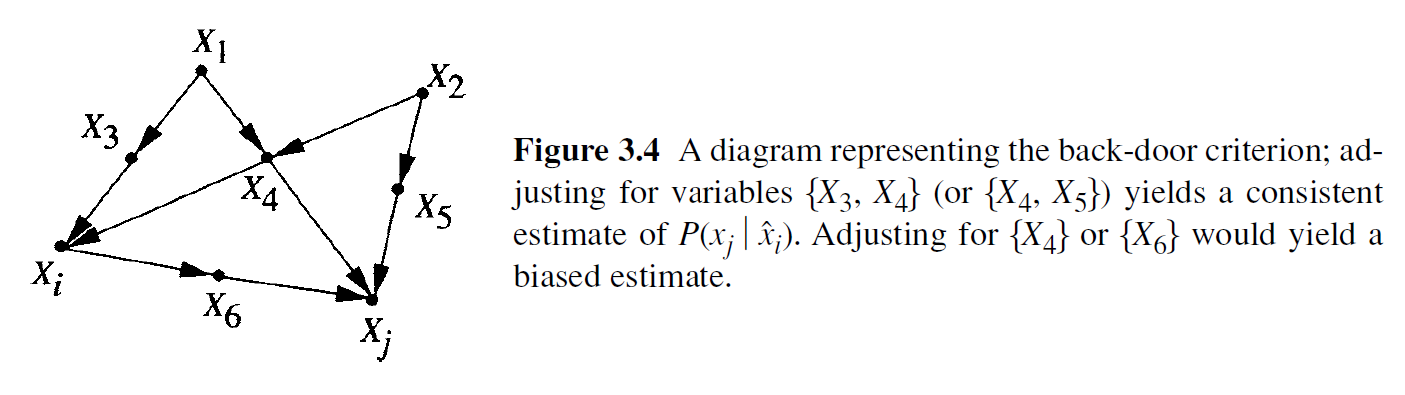
\includegraphics[width=0.8\columnwidth]{figures/back-door.png}  
\end{center}
\caption{Example of the back-door criterion
}
\label{Fig:front_door}
\end{figure}

\begin{defn}[Back-door criterion] A set of variables $Z$ satisfy the back-door criterion relative to an ordered pair of variables ($X_i$,$X_j$) in a DAG $G$ if:
\begin{enumerate}[noitemsep]
\item no node in $Z$ is a descendant of $X_i$; and
\item $Z$ blocks every path between $X_i$ and $X_j$ that contains an arrow into $X_i$
\end{enumerate}
Similarly, if $X$ and $Y$ are two disjoint subsets of nodes in $G$, then $Z$ satisfies the back-door criterion relative to $(X,Y)$ if it satisfies the criterion relative to any pair $(X_i, X_j)$ such that $X_i \in X$ and $X_j \in Y$.
\end{defn}

\begin{thm}[Back-door adjustment]
If a set of variables $Z$ satisfies the back-door criterion relative to $(X,Y)$, then the causal effect of $X$ on $Y$ is identifiable and is given by
\begin{equation}
P(y|\hat{x}) = \sum_z P(y|x,z)P(z).
\end{equation}
This corresponds to partitioning the population into groups that are homogeneous relative to $Z$, assessing the effect of $X$ on $Y$ in each homogeneous group, and then averaging the results. Conditioning in this way means that the observation $X=x$ cannot be distinguished from an intervention $do(x)$. \label{thm:back-door-adjustment}
\end{thm}

\subsection{The front-door criterion}
This criterion demonstrates how confounders that are \textit{affected by} the treatment variable can be used to facilitate causal inference.

\begin{figure}
\begin{center}
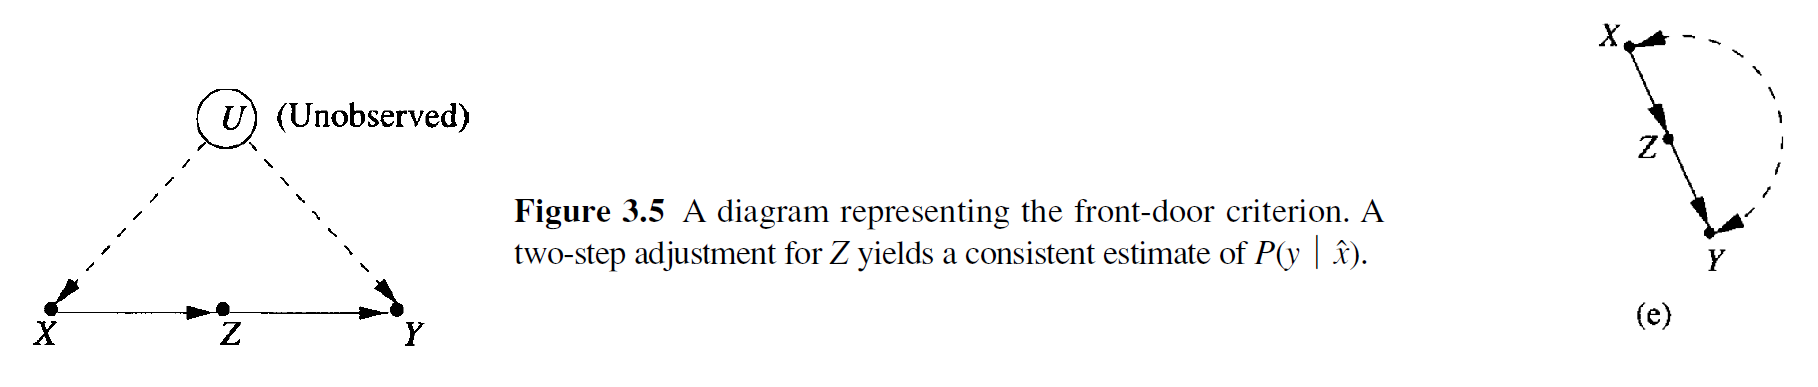
\includegraphics[width=0.8\columnwidth]{figures/front-door.png}  
\end{center}
\caption{(Left) Example of the front-door criterion. The path $X \leftarrow U \rightarrow Y$ denotes an unobserved (latent) unobserved common cause. (Right) This is often represented as a \textbf{bi-directed path}. 
}
\label{Fig:front_door}
\end{figure}

\begin{defn}[Front-door]
A set of variables $Z$ satisfy the front-door criterion relative to an ordered pair of variables $(X, Y)$ if:
\begin{enumerate}[noitemsep]
\item $Z$ intercepts all directed paths from $X$ to $Y$; 
\item there is no unblocked back-door path from $X$ to $Z$; and
\item all back-door paths from $Z$ to $Y$ are blocked by $X$.
\end{enumerate}
\end{defn}

\begin{thm}[Front-door adjustment]
If $Z$ satisfies the front-door criterion relative to $(X, Y)$ and if $P(x, z) > 0$, then the causal effect of $X$ on $Y$ is identifiable and is given by
\begin{equation}
P(y|\hat{x}) = \sum_z P(z|x) \sum_{x'} P(y|x',z)P(x')
\end{equation}
\end{thm}

Conditions (2) and (3) of the front-door definition are overly restrictive: e.g. nested combinations of back-door and front-door conditions are permissible: see Section~\ref{sec:do-calc} for a more general set of conditions.

\section{Do-calculus} \label{sec:do-calc}

The back-door and front-door criteria do not provide a complete set of rules for when/how causal effects can be computed. Do-calculus sidesteps the need for algebraic manipulation and provides a complete set of inference rules by which probabilistic sentences involving interventions and observations can be transformed into other such sentences, allowing a method of deriving/verifying claims about interventions. The aim is to compute causal effect expressions for $P(y|\hat{x})$ where $Y$ and $X$ are subsets of variables. When $P(y|\hat{x})$ can be reduced to an expression involving observable probabilistic quantities, we say that the causal effect of $X$ on $Y$ is \textbf{identifiable}.

\subsection{Notation}
\begin{itemize}[noitemsep]
\item $G_{\overline{X}}$ = graph obtained by deleting from $G$ all arrows pointing into nodes in $X$
\item $G_{\underline{X}}$ = graph obtained by deleting from $G$ all arrows pointing out of nodes in $X$
\item $G_{\overline{X}\underline{Z}}$ = graph obtained by deleting from $G$ all arrows pointing into nodes in $X$ and out of nodes in $Z$
\item $P(y|\hat{x},z) \defeq P(y,z|\hat{x}) / P(z|\hat{x})$, meaning the probability of observing $Y=y$ given an \textit{intervention} $X=x$ and an \textit{observation} $Z=z$
\end{itemize}

\subsection{Rules} \label{sec:Rules}

\begin{rle}[Insertion/deletion of observations] 
\begin{equation}
P(y|\hat{x}, z, w) = P(y| \hat{x}, w) \quad \text{if}\ (Y \indep Z|X,W)_{G_{{\overline{X}}}}.
\end{equation} \label{rle:do-calc-ins-del-obs}
\end{rle}

Rule~\ref{rle:do-calc-ins-del-obs} is a reaffirmation of $d$-separation (Section~\ref{sec:blocking}) as a valid test for conditional independence in the distribution resulting from $do(X=x)$. The rule follows from the fact that deleting equations from the system ($G_{{\overline{X}}}$) does not introduce any dependencies among the remaining disturbance terms.

\begin{rle}[Action/observation exchange]
\begin{equation}
P(y|\hat{x},\hat{z},w) = P(y|\hat{x},z,w) \quad \text{if}\ (Y \indep Z|X,W)_{G_{{\overline{X}\underline{Z}}}}.
\end{equation}  \label{rle:do-calc-act-obs-ex}
\end{rle}

Rule~\ref{rle:do-calc-act-obs-ex} provides a condition for an external intervention $do(Z=z)$ to have the same effect on $Y$ as the passive observation $Z=z$. The condition amounts to $\{X \cup W\}$ blocking all back-door paths from $Z$ to $Y$ (in $G_{\overline{X}}$), since $G_{\overline{X}\underline{Z}}$ retains all (and only) such paths.

\begin{rle}[Insertion/deletion of actions] 
\begin{equation}
P(y|\hat{x},\hat{z},w) = P(y|\hat{x},w) \quad \text{if}\ (Y \indep Z|X,W)_{G_{{\overline{X},\overline{Z(W)}}}}
\end{equation}  \label{rle:do-calc-ins-del-act}
where $Z(W)$ is the set of $Z$-nodes that are not ancestors of any $W$-node in $G_{\overline{X}}$.
\end{rle}

Rule~\ref{rle:do-calc-ins-del-act} provides conditions for introducing (or deleting) an external intervention $do(Z=z)$ without affecting the probability of $Y=y$. The validity of this rule stems from simulating the intervention $do(Z=z)$ by the deletion of all equations corresponding to the variables in $Z$ (hence $G_{\overline{X} \overline{Z}}$).

\paragraph{Completeness} A quantity $Q=P(y|do(x),z)$ is identifiable if and only if it can be reduced to a \textit{do}-free expression using the above 3 rules.

\subsection{Identifiability}
A causal effect $q = P(y_1, \dots, y_k| \hat{x}_1, \dots, \hat{x}_m)$ is identifiable in a model characterised by a graph $G$ if there exists a finite sequence of transformations conforming to one of the three rules in Section~\ref{sec:Rules} that reduces $q$ into a standard (i.e.\ ``hat''-free) probability expression involving observed quantities. Figure \ref{Fig:graph_cond_ci} provides a set of graphical conditions; if any one is satisfied then $P(y|\hat{x})$ is identifiable, and satisfying at least one of the conditions is necessary for $P(y|\hat{x})$ to be identifiable. I.e. $P(y|\hat{x})$ is unidentifiable then no finite sequence of inference rules reduces $P(y|\hat{x})$ to a hat-free expression. Figure \ref{Fig:graph_cond_ci} can also be used to define an algorithm for deriving a closed-form expression for control queries in terms of observable quantities, see Section~\ref{sec:soft-causaleffect} for an implementation.


\begin{figure}
\begin{center}
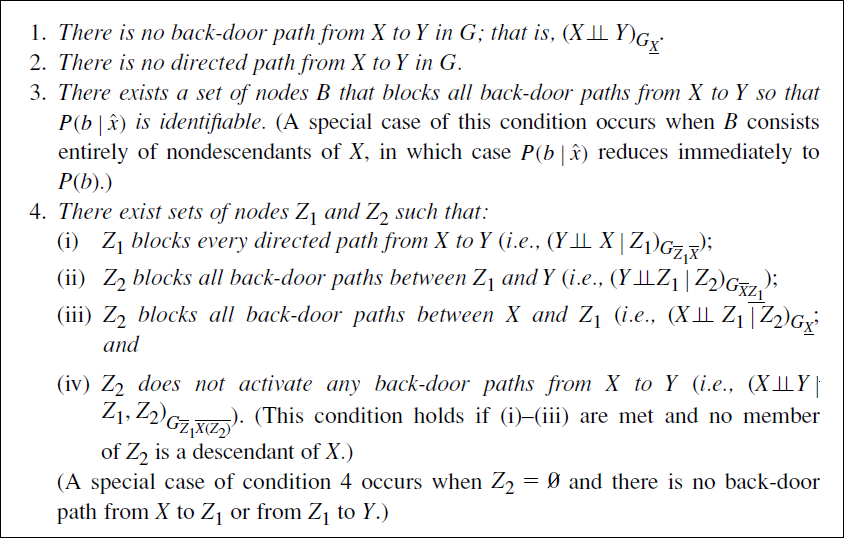
\includegraphics[width=0.8\columnwidth]{figures/graph-cond-ident-4-3-1.png}  
\end{center}
\caption{Graphical conditions for identification of causal effect (Theorem 4.3.1 Causality). Satisfying at least one renders the causal effect $P(y|\hat{x})$ identifiable, whereas satisfying none implies unidentifiability of the causal effect.}
\label{Fig:graph_cond_ci}
\end{figure}

\paragraph{Assorted facts on identifiability} 

\begin{itemize}
\item Whilst a causal effect is not identifiable for \textit{every} joint distribution of variables if this condition is broken, it might be for \textit{some} probability densities. For example, an instrumental variable can yield a causal effect identifiable in a linear model in the the presence of a bow pattern (Fig.~3.7A of Causality), but will not be generally identifiable (see Section 3.5 of Causality).
\item If $P(y|\hat{x})$ is identifiable, then if a set of nodes $Z$ lies on a directed path from $X$ to $Y$, then $P(z|\hat{x})$ is also identifiable (lemma 4.3.4).
\end{itemize}

\begin{defn}[$d$-separation equivalence] \label{defn:d-sep-equiv}
For two nodes $a$ and $b$ in a causal diagram $M$, we write $a \underset{M}{\text{---}} b$ if $a$ and $b$ are adjacent in model $M$. We write conditional adjacency $a \underset{M}{\text{---}} b | c$ to mean once given $c$, $a$ and $b$ cannot be independent: graphically, $a$ and $b$ are the common parents of $c$, or some ancestor of $c$, or $a$ and $b$ are unconditionally adjacent.  Two causal models $D$ and $E$ over the set of nodes $N$, are d-separation equivalent if \citep{Verma88}:
\begin{align}
\underset{a,b \in N}{\forall} a \underset{D}{\text{---}} b &\iff a \underset{E}{\text{---}} b \\
\underset{a,b \in N}{\forall} a \underset{D}{\text{---}} b | c &\iff a \underset{E}{\text{---}} b | c
\end{align}
\end{defn}

\begin{cor}\label{cor:d-sep-equiv-thm}
If models $D$ and $E$ are $d$-separation equivalent (see Definition~\ref{defn:d-sep-equiv}), then they are observationally equivalent: i.e. they are unidentifiable from each other. 
\end{cor}

\begin{thm}[Complete identifiability condition]
A sufficient condition for identifying the causal effect $P(y|do(x))$ is that there exists no bi-directed path (i.e.\ a path composed entirely of bi-directed arcs, see Fig.~\ref{Fig:front_door}) between $X$ and any of its children \citep{Tian02}. Prior to applying this criterion, all nodes which are not ancestors of $Y$ are deleted from the graph (i.e.\ only consider nodes which are on pathways from $X$ to $Y$).
\end{thm}

\subsection{Confounders, latent common causes, and bi-directed arcs}

Bi-directed arcs are, by definition, equivalent to a latent common cause (also known as a confounder) between the two connecting variables (see Fig.~\ref{Fig:confounders}). This notation is useful because it is the only triad with a single latent variable where the latent common cause renders the causal effect unidentifiable. In Fig.~\ref{Fig:confounders}B, even if $U$ were available, conditioning upon it would induce collider bias. In Fig.~\ref{Fig:confounders}C, it is intuitive that $U$ is unnecessary to be known, because all causal effects are mediated by a very large number of unobserved causes, but we do not need complete knowledge of the world to make causal inferences.


\begin{figure}
\begin{center}
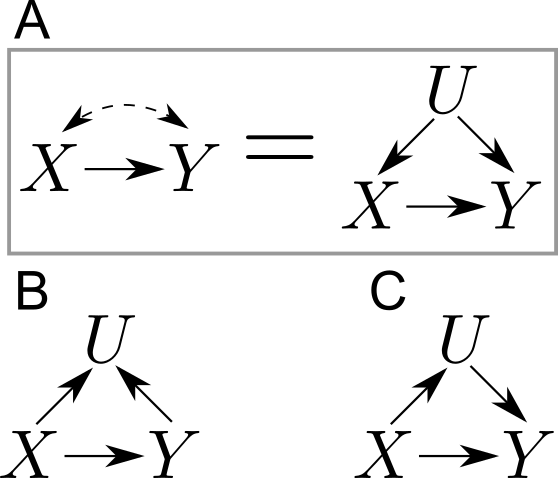
\includegraphics[width=0.4\columnwidth]{figures/confounders.png}  
\end{center}
\caption{\textbf{Bi-directed arcs are latent common causes by definition, and are the only acyclic triad with an unobserved variable where the causal effect is unidentifiable}. A) A bi-directed arc between variables $X$ and $Y$ is, by definition, equivalent to the graph $U \rightarrow X \rightarrow Y \leftarrow U$ where $U$ is unobserved (latent). This notation is useful because this triad is unique, in the sense that it is the only possible triad involving $U$ where $P(Y|do(x))$ is unidentifiable. B) For this DAG, applying Theorem~\ref{thm:do-calc-act-obs-ex}, $P(Y|do(x)) = P(Y|X)$, and so $U$ is irrelevant for estimation of the causal effect.  C) Again, $P(Y|do(x)) = P(Y|X)$ so $U$ is irrelevant. The final permutation of arrows is omitted because it induces a cycle, which is beyond the scope of basic causal inference.} 
\label{Fig:confounders}
\end{figure}


\section{Actions, plans, and direct effects}

Pearl defines two kinds of intervention:

\begin{itemize}[noitemsep]
\item Act: An intervention which results from a reactive policy, deriving from an agent's beliefs, disposition, and environmental inputs (or the ``outside'')
\item Action: An intervention which results from a deliberative policy, deriving from an agent's free will (or the ``inside''; meditative traditions might not draw such a bright line between these two classifications as a  description of physical reality, but it is no doubt a useful distinction for reasoning about the future when conscious agents are involved)
\end{itemize} 

\subsection{Conditional actions and stochastic policies}
In general, interventions may involve complex policies in which $X$ is made to respond according to e.g. a deterministic functional relationship $x=g(z)$, or more generally through a stochastic relationship whereby $X$ is set to $x$ with probability $P^*(x|z)$. 


Let $P(y|do(X=g(z)))$ denote the distribution of $Y$ prevailing under the deterministic policy $do(x=g(z))$. Then,
\begin{align}
P(y|do(X=g(z))) &= \sum_z P(y|do(X=g(z)),z) P(z|do(X=g(z))) \\
&= \sum_z P(y|\hat{x}, z)|_{x=g(z)} P(z) \nonumber \\
&= E_z[P(y|\hat{x},z)|_{x=g(z)}]. \nonumber
\end{align}
Hence, the evaluation of the outcome of an intervention under a complicated conditional policy $x=g(z)$ amounts to being able to evaluate $P(y|\hat{x},z)$. The equality $P(z|do(X=g(z))) = P(z)$ stems from the fact that $Z$ \textbf{cannot} be a descendant of $X$: in other words, \textbf{one cannot define a coherent policy of action for $X$ based on an (indirect) effect of $X$ because actions change the distributions of their effects!} (Aside: I suppose one might argue about whether an agent has any choice over the form of $g(z)$)

Similarly, let $P(y)|_{P^*(x|z)}$ denote the distribution of $Y$ prevailing under the stochastic policy $P^*(x|z)$ -- i.e.\ given $Z=z$, $do(X=x)$  occurs with probability $P^*(x|z)$. Then,
\begin{equation}
P(y)|_{P^*(x|z)} = \sum_x \sum_z P(y|\hat{x}, z) P^*(x|z) P(z).
\end{equation}
Since $P^*(x|z)$ is specified externally, it is again the case that $P(y|\hat{x}, z)$ is sufficient for the identifiability of any stochastic policy which shapes the distribution of $X$ by the outcome of $Z$.


\subsection{Identification of dynamic plans}

A \textbf{control problem}  consists of a DAG with vertex set $V$ partitioned into four disjoint sets $V=\{X,Z,U,Y\}$ where
\begin{itemize}
\item $X=$ the set of control variables (exposures, interventions, treatments, etc.)
\item $Z=$ the set of observed variables, often called \textbf{covariates}
\item $U=$ the set of unobserved (latent) variables, and
\item $Y=$ an outcome variable
\end{itemize}
We are interested in settings where we have gathered data $\mathcal{D}=\{X,Z,Y\}$ for previous agents making actions $X$. The problem is, given a new instance of the system (e.g.\ a new patient whom we seek to treat), can we estimate the outcome of $\{do(x_1),...,do(x_n)\}$ using only the observational data $\mathcal{D}$. See Section 4.4.1 of Causality for a specific motivating example.

Let control variables be ordered $X=X_1,...,X_n$ such that every $X_k$ is a non-descendant of $X_{k+j}$ ($j>0$) and let the outcome $Y$ be a descendant of $X_n$. A \textbf{plan} is an ordered sequence $(\hat{x}_1,...,\hat{x}_n)$ of value assignments to the control variables. A \textbf{conditional plan} is an ordered sequence $(\hat{g}_1(z_1),...,\hat{g}_n(z_n))$ where $\hat{g}_k(z_k)$ means ``set $X_k$ to $\hat{g}_k(z_k)$ whenever $Z_k=z_k$'', where the support $Z_k$ of each $g_k(z_k)$ must not contain any variables that descendants of $X_k$.

\begin{thm}[Plan identification: the sequential back-door criterion]
The probability of the \textbf{unconditional} plan $P(y|\hat{x_1}, ..., \hat{x}_n)$ is identifiable if, for every $1 \leq k \leq n$ there exists a set $Z_k$ of covariates satisfying the following conditions:
\begin{equation}
Z_k \subseteq N_k
\end{equation}
where $N_k$ is the set of observed nodes that are non-descendants of any element of $\{X_k, X_{k+1},...,X_n\}$, and
\begin{align}
(Y \indep X_k | X_1,...,X_{k-1},Z_1,...,Z_k)_{{G_{\underline{X}_k,\overline{X}_{k+1},...,\overline{X}_{n}}}}
\end{align}
When these conditions are satisfied, the effect of the plan is given by
\begin{align}
P(y|\hat{x}_1,...,\hat{x}_n) = \sum_{z_1,...,z_n} P(y|z_1,...,z_n,x_1,...,x_n) \times \prod_{k=1}^n P(z_k|z_1,...,z_{k-1},x_1,...,x_{k-1})
\end{align}
\end{thm}

\subsection{Direct and indirect effects}

We are often concerned with the extent to which a variable affects another directly, rather than the total causal effect mediated through all other intervening variables. For example, in cases of sex discrimination, we may be interested in asking the direct effect of an applicant's sex on the outcome of an applicant's job application. In effect, we are concerned with the causal effect of variable $X$ on $Y$ while all other factors in the analysis are held fixed (\textit{Ceteris paribus}).

\begin{defn}[Direct effect]
The direct effect of $X$ on $Y$ is given by $P(y|\hat{x},\hat{s}_{XY})$ where $\hat{s}_{XY}$ is the set of all variables in the model except $X$ and $Y$
\end{defn}

\begin{cor}
The direct effect of $X$ on $Y$ is given by $P(y|\hat{x}, \hat{pa}_{Y \setminus X})$ where $pa_{Y \setminus X}$ is any realization of the parents of $Y$ excluding $X$.
\end{cor}

It is sometimes meaningful to average the direct effect over all levels of $pa_{Y\setminus X}$. To do this, we define the natural direct effect:

\begin{defn}[Natural direct effect]
The natural direct effect ($DE_{x,x'}(Y)$) is defined as
\begin{equation}
DE_{x,x'}(Y) \defeq E[Y(x', Z(x)) - E(Y(x))]
\end{equation}
where $Z= pa_{Y\setminus X}$, and $Y(x', Z(x))$ is the value that $Y$ would attain under the counterfactual scenario of $X=x'$, but $Z$ retaining the values under the setting $X=x$.
\end{defn}

The natural direct effect involves probabilities of nested counterfactuals, and cannot generally be written in terms of the $do(x)$ operator. However, if certain assumptions of ``no confounding'' are deemed valid, the natural direct effect can be reduced to 

\begin{equation}
DE_{x,x'}(Y) = \sum_z [E(Y|do(x', z)) - E(Y| do(x,z))]P(z|do(x))
\end{equation}
which is simply a weighted average of controlled direct effects. 

We can also define the indirect effect which quantifies the influence of $X$ on $Y$ through all paths except for the direct path from $X \rightarrow Y$.
\begin{defn}[Indirect effect]
The natural indirect effect ($IE_{x,x'}(Y)$) is defined as
\begin{equation}
IE_{x,x'}(Y) = E[Y(x, Z(x')) - E(Y(x))]
\end{equation}
\end{defn}
We can define 
\begin{defn}[Total effect] 
The total effect of $X$ on $Y$ is given by $P(y|do(x))$, namely, the distribution of $Y$ while $X$ is held constant at $x$ and all other variables are permitted to run their natural course.  \textbf{Confusingly}, we also sometimes denote the total effect $TE_{x,x'}(Y)$ as 
\begin{equation}
TE_{x,x'}(Y) \defeq E[Y(x') - E(Y(x))] 
\end{equation}
\textbf{TODO: Write $TE_{x,x'}(Y)$ in terms of $P(y|do(x))$? Is it $E(y|do(x')) - E(y|do(x))$?}
\end{defn}

\begin{thm}[Relationship between total effect, direct effect, and indirect effect]
The total effect of a transition is the \textit{difference} between the direct effect of that transition and the indirect effect of the reverse transition
\begin{equation}
TE_{x,x'}(Y) = DE_{x,x'}(Y) - IE_{x',x}(Y)
\end{equation}
\end{thm}

\section{Causality and structural models}

Let's rewrite Eq.\eqref{eq:func-caus-mod} as
\begin{equation}
x_i = f_i(pa_i, \epsilon_i), \quad i=1,...,n. 
\end{equation}
In general, for the \textbf{partial correlation} $\rho_{XY\cdot Z}$, 
\begin{equation}
(X \indep Y | Z) \implies \rho_{XY\cdot Z} = 0 
\end{equation}
and therefore, in \textbf{any} Markovian model with DAG $G$, the partial correlation $\rho_{XY\cdot Z}$ vanishes whenever the nodes corresponding to the variables in $Z$ $d$-separate node $X$ from node $Y$ in $G$, regardless of model parameters. Moreover, no other partial correlation vanishes, for all model parameters. \textbf{[Q: Not sure if this is general or only for linear models]}

\begin{thm}[Test for correlation between error terms]
For any two non-adjacent variables $X$ and $Y$, where $Y$ is \textbf{not} a parent of $X$, a sufficient test of whether $\epsilon_X$ and $\epsilon_Y$ are uncorrelated is if the following equality holds:
\begin{equation}
E[Y|x,do(S_{XY})] = E[Y|do(x),do(S_{XY})] \label{eq:test-corr-error}
\end{equation}
where $S_{XY}$ stands for (any setting of) all variables in the model excluding $X$ and $Y$. If $\epsilon_X$ and $\epsilon_Y$ are uncorrelated then we are justified in having the absence of a bidirected arc between $X$ and $Y$. I.e.\ the omitted factors which directly affect $X$, $\epsilon_X$, are independent of the omitted factors which directly affect $Y$, $\epsilon_Y$.
\end{thm}

\begin{figure}
\begin{center}
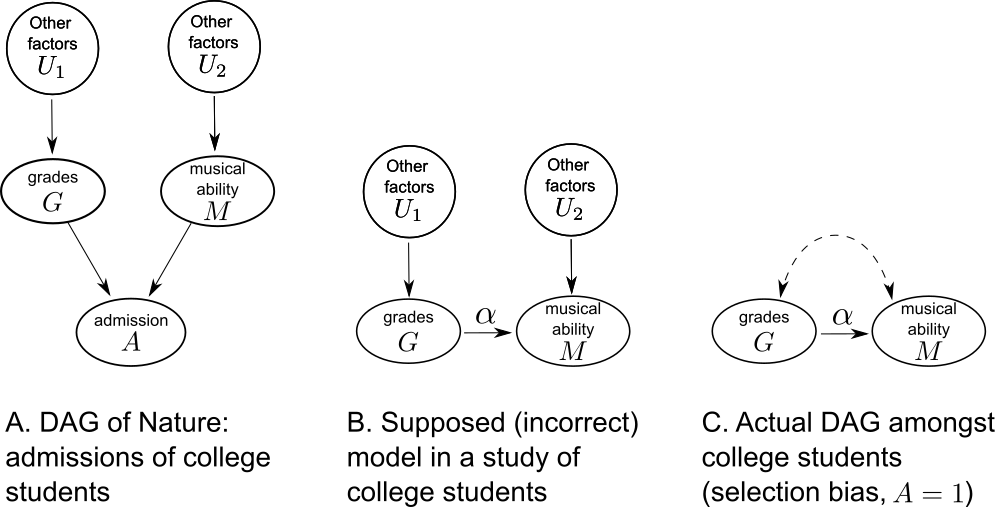
\includegraphics[width=0.8\columnwidth]{figures/selection-bias.png}  
\end{center}
\caption{\textbf{An example of selection bias in a study}. A) Suppose, for a particular college, both grades and musical ability affect admission rate. B) Suppose investigators seek to understand the relationship between grades and musical ability, and measure $G$ and $M$ amongst students of the college in an attempt to estimate $\alpha$ ($\alpha=0$ in reality). The investigators assume the DAG in (B) and discover a strong negative relationship between $G$ and $M$. C) However, the investigators would discover that the equality in Eq.\eqref{eq:test-corr-error} does not hold, and therefore $U_1$ and $U_2$ are correlated (owing to a selection bias from $A=1$, see Berkson's paradox). Hence the investigators should correct their DAG to include a latent common cause between $G$ and $M$ in order to prevent spurious inferences (see Fig.~\ref{Fig:confounders}). In doing so, $\alpha$ becomes unidentifiable since all of the causal effect can (and, here, is!) attributable to selection bias.}
\label{Fig:selection-bias}
\end{figure}

Note that \textbf{selection bias} can arise when two uncorrelated factors have a common effect that is omitted from the analysis but influences the selection of samples for the study, see Fig.~\ref{Fig:selection-bias}. Hence bidirected arcs should be assumed to exist, by default, between any two nodes in a diagram -- since they at worst compromise the identifiability of model parameters. They should be deleted only by well-motivated justifications, such as the unlikely existence of a common cause, and the unlikely existence of selection bias.

\subsection{Exogeneity} \label{sec:exogeneity}

\begin{defn}[General Exogeneity]
Let $X$ and $Y$ be two sets of variables, and let $\lambda$ be any quantity which may be computed from a structural model $M$ (structural, statistical, etc.) in a theory $T$. We say that $X$ is exogenous relative to $(Y, \lambda ,T)$ if $\lambda$ is identifiable from the conditional distribution of $P(y|x)$, that is, if
\begin{equation}
P_{M_1}(y|x) = P_{M_2}(y|x) \implies \lambda(M_1) = \lambda(M_2)
\end{equation}
for any two models $M_1$ and $M_2$ satisfying theory $T$. \label{def:general-exog}
\end{defn}

The following three alternative definitions of exogeneity are also sometimes given, but are not generally equivalent when we cannot assume stability. In order of decreasing strength:
\begin{defn}[Graphical criterion for exogeneity]
A variable $X$ is exogenous in model $M$ relative to $Y$ if $X$ and $Y$ have no common ancestor in $G(M)$ or, equivalently, if all back-door paths between $X$ and $Y$ are blocked (by colliding arrows). ``Common ancestors'' should exclude nodes that have no other connection to $Y$ except through $X$, but should include latent nodes for every pair of dependent errors.
\end{defn}
\begin{defn}[Error-based criterion for exogeneity]
A variable $X$ is exogenous in model $M$ relative to $Y$ if $X$ is independent of all error terms ($U$ in Defn.~\ref{defn:struct-causal-model}) that have an influence on $Y$ when $X$ is held constant. I.e. A variable $X$ is exogenous relative to $\lambda=P(y|do(x))$ if $X$ is independent of all errors $U$ that influence $Y$, except those mediated by $X$.
\end{defn}
\begin{defn}[Empirical criterion for exogeneity]
A variable $X$ is exogenous relative to $Y$ if and only if 
\begin{equation}
P(Y_x=y)=P(y|x)
\end{equation}
(see Section~\ref{sec:counterfactual-defs} for definitions of counterfactuals), or equivalently
\begin{equation}
P(Y=y|do(x))=P(y|x)
\end{equation}
\end{defn}
\noindent where
\begin{equation}
\text{graphical criterion} \implies \text{error-based criterion} \implies \text{counterfactual criterion}.
\end{equation}
However, if we assume stability, then the three definitions coincide.

\subsection{Instrumental variables}
\begin{defn}[Instrumental variable]
For the parameter $\lambda = P(w|do(z))$ where $W$ and $Z$ are two sets of variables in $Y$, then if $X$ is exogenous relative to $(Y, \lambda, T)$ then
\begin{equation}
P_{M_1}(z,w|x) = P_{M_2}(z,w|x) \implies P_{M_1}(w|do(z)) = P_{M_2}(w|do(z)).
\end{equation}
for any two models $M_1$ and $M_2$ satisfying theory $T$. Under these conditions, we call $X$ an instrumental variable for the causal effect $P(w|do(z))$
\end{defn}

\begin{cor}
If $X$ is an instrumental variable for $P(w|do(z))$, then $P(w|do(z))$ is identifiable from $P(z,w|x)$. I.e. $X$ renders a causal effect $P(w|do(z))$ identifiable which $X$ itself does not directly participate in.
\end{cor}

As in the case of exogeneity, we can provide graphical and counterfactual criteria for instrumental variables
\begin{defn}[Criteria for instrumental variables]
A variable $Z$ is an instrument relative to the total effect of $X$ on $Y$ if there exists a set of measurements $S=s$ (i.e. joint observations for $X$, $Y$, and $Z$? \textbf{[TODO: Confirm?]}), unaffected by $X$, such that either of the following criteria holds
\begin{enumerate}
\item \textbf{Counterfactual} criterion
\begin{enumerate}
\item $Z \indep Y_x | S=s$
\item $Z \nindep X|S=s$
\end{enumerate}
\item \textbf{Graphical} criterion
\begin{enumerate}
\item $(Z \indep Y|S)_{G_{\bar{X}}}$
\item $(Z \nindep X|S)_G$
\end{enumerate}
\end{enumerate} 
\end{defn}


\subsection{Linear structural equation models}

Linear structural equation models (SEMs) obey
\begin{equation}
x_i = \sum_{k \neq i} \alpha_{ik} x_k + \epsilon_i, \quad i=1,...,n  \label{eq:linear_sem}
\end{equation}
If, in Eq.\eqref{eq:linear_sem} 
\begin{equation}
\epsilon \sim \mathcal{N}(\mu, \Sigma)
\end{equation}
then $X_i$ will also be multivariate normal, and the SEM will be entirely determined by the set of correlation coefficients $\rho_{ij}$. For a linear SEM
\begin{equation}
\rho_{XY\cdot Z} = 0 \iff (X \indep Y | Z).
\end{equation}


\subsubsection{Interpretation}

\begin{defn}[Structural equations]
An equation 
\begin{equation}
y=\beta x + \epsilon \label{eq:linear-struct}
\end{equation}
is said to be structural if it is to be interpreted as follows: In an ideal experiment where we control $X$ to $x$ and any other set $Z$ of variables (not containing $X$ or $Y$) to $z$, the value of $Y$ is given by $\beta x + \epsilon$, where $\epsilon$ is not a function of the settings $x$ and $z$. \textbf{[I think: $\epsilon$ can be arbitrarily distributed, potentially correlated with $X$, but assumed to have $E[\epsilon]=0$.]}
\end{defn}

The equality sign in structural equations has a different behaviour to algebraic equality signs. In the context of observations, the equality sign in Eq.\eqref{eq:linear-struct} behaves symmetrically between $X$ and $Y$: e.g.\ observing $Y=0$ implies $\beta x = -\epsilon$. In contrast, in the context of interventions, the equality sign in Eq.\eqref{eq:linear-struct} behaves asymmetrically between $X$ and $Y$: e.g.\ setting $Y=0$ tells us nothing about the relationship between $x$ and $\epsilon$. 

Furthermore, the strongest empirical claim made by Eq.\eqref{eq:linear-struct} is that
\begin{equation}
P(y|do(x), do(z)) = P(y|do(x))
\end{equation}
i.e.\ the statistics of $Y$ remain invariant to the manipulation of $Z$ under the condition of $do(x)$. In contrast, regression equations make no empirical claims whatsoever.

The operational definition of the structural parameter $\beta$ in Eq.\eqref{eq:linear-struct} is
\begin{equation}
\beta = \frac{\partial}{\partial x}E[Y|do(x)]
\end{equation}
(since $E[Y|do(x)]=\beta x$). In words, $\beta$ is the rate of change in the expectation of $Y$ in an experiment where $X$ is held at $x$ by external control. This is true regardless of the correlation between $X$ and $\epsilon$ in non-experimental studies (e.g.\ via another equation $x=\alpha y + \delta$).

As a consequence of the above, the operational definition of the error term $\epsilon$ is
\begin{equation}
\epsilon = y - E[Y|do(x)]
\end{equation}
(again since $E[Y|do(x)]=\beta x$). 

\subsubsection{Estimation}

Define the conditional variance $\sigma^2_{X|z}$, conditional covariance $\sigma^2_{XY|z}$, and the conditional covariance $\rho_{XY|z}$. For multivariate normal, $\sigma^2_{X|z}$, $\sigma^2_{XY|z}$, and $\rho_{XY|z}$ are all independent of the value of $z$. For the MVN, the \textbf{partial} variance $\sigma^2_{X\cdot Z}$, covariance $\sigma_{XY\cdot Z}$, and correlation $\rho_{XY\cdot Z}$ all coincide with the conditional variance, covariance, and correlation respectively (although this is not generally the case). 

A \textbf{partial regression coefficient}, $r_{YX\cdot Z}$ is given by
\begin{equation}
r_{YX\cdot Z} = \rho_{YX\cdot Z} \frac{\sigma_{Y\cdot Z}}{\sigma_{X\cdot Z}}
\end{equation}
and is equal to the coefficient of $X$ in the linear regression of $Y$ on $X$ and $Z$. So, the coefficient of $x$ in the regression equation
\begin{equation}
y = \alpha x + b_1 z_1 +...+ b_k z_k
\end{equation}
is
\begin{equation}
\alpha=r_{YX\cdot Z_1Z_2...Z_k}
\end{equation}

\begin{thm}[$d$-Separation in General Linear Models]
For any linear model Eq.\eqref{eq:linear_sem}, which may include cycles and bidirected arcs (i.e. dependent $\epsilon$ between different variables), $\rho_{XY\cdot Z}=0$ if $Z$ d-separates $X$ from $Y$, where bidirected arcs between $i$ and $j$ are interpreted as a latent common parent $i \leftarrow L \rightarrow j$. \label{thm:d-sep-lin-model}
\end{thm}

Theorem \ref{thm:d-sep-lin-model} provides a method for finding models in the context of linear SEMs: by searching over all $\rho_{XY\cdot Z}$, we can construct a DAG. Not all partial correlations need to be searched.

\begin{defn}[Basis]
Let $S$ be a set of partial correlations. A basis $B$ for $S$ is a set of zero partial correlations where (i) $B$ implies the zero of every element of $S$ and (ii) no proper subset of $B$ sustains such an implication.
\end{defn}

An obvious choice of basis for a DAG $D$ is
\begin{equation}
B = \{\rho_{ij\cdot pa_{i}} | i>j \} 
\end{equation}
where $i$ ranges over all nodes in $D$ and $j$ ranges over all predecessors of $i$ in any order that agrees with the arrows of $D$. More economical choice of basis exist, such as a Graphical Basis. 

\begin{thm}[Markov linear-normal equivalence]
Two Markovian linear-normal models are observationally indistinguishable if every covariance matrix generated by one model can be parametrically generated by the other (covariance equivalent). Two such models are covariance equivalent if and only if their corresponding graphs have the same sets of zero partial correlations. Moreover, two such models are covariance equivalent if and only if they have the same edges and the same sets of $v$-structures. (I.e. arrows can be reversed as long as they do not alter $v$-structures, see Corollary~\ref{cor:d-sep-equiv-thm}).
\end{thm}


\subsubsection{Parameter identifiability}

Consider an edge $X \rightarrow Y$ in graph $G$, and let $\alpha$ be the path coefficient associated with that edge (i.e. the strength of the direct causal effect of $X$ on $Y$). The regression coefficient in a linear model can, in general, be decomposed into 
\begin{equation}
r_{YX} = \alpha + I_{YX}
\end{equation}
where $I_{YX}$ is independent of $\alpha$, since $I_{YX}$ is composed of other indirect paths connecting $X$ and $Y$. If we remove the edge $X \rightarrow Y$ and observe that the resulting subgraph entails zero correlation between $X$ and $Y$ then $I_{XY}=0$ and $r_{YX}=\alpha$, and hence $\alpha$ is identified. This idea is extended in the following theorem
\begin{thm}[Single-door Criterion for Direct Effects] 
Let $G$ be any path diagram in which $\alpha$ is the path coefficient associated with link $X \rightarrow Y$, and let $G_\alpha$ denote the diagram that results when $X\rightarrow Y$ is deleted from $G$. The coefficient $\alpha$ is identifiable if there exists a set of variables $Z$ such that (i) $Z$ contains no descendant of $Y$ and (ii) $Z$ d-separates $X$ from $Y$ in $G_\alpha$. If $Z$ satisfies these two conditions then, in a linear SEM, $\alpha = r_{YX\cdot Z}$. Conversely, if $Z$ does not satisfy these conditions, then $r_{YX\cdot Z}$ is not a consistent estimand of $\alpha$. \label{thm:single-door-direct-effect}
\end{thm}

\begin{thm}[Back-door Criterion for Total Effects]
For any two variables in a causal diagram $G$, the total effect of $X$ on $Y$ is identifiable if there exists a set of measurements $Z$ such that 
\begin{enumerate}
\item no member of $Z$ is a descendant of $X$; and
\item $Z$ d-separates $X$ from $Y$ in the subgraph $G_{\underline{X}}$ formed by deleting all $G$ arrows emanating from $X$
\end{enumerate}
If the two conditions are satisfied, then the total effect of $X$ on $Y$ in a linear SEM is given by $r_{YX\cdot Z}$. \label{thm:back-door-total-effect}
\end{thm}

Theorems \ref{thm:single-door-direct-effect} and \ref{thm:back-door-total-effect} are special cases of a more general scheme. In order to identify any \textbf{partial effect}, as defined by a select bundle of causal paths from $X$ to $Y$, we must find a set $Z$ of measured variables that block all non-selected paths between $X$ and $Y$. For linear models, the partial effect is equal to the regression coefficient $r_{YX\cdot Z}$.

\begin{figure}
\begin{center}
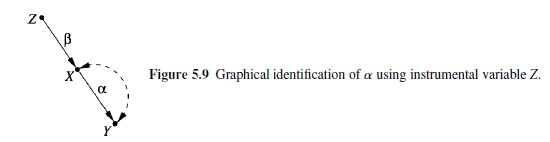
\includegraphics[width=0.8\columnwidth]{figures/instrumental-variable.jpg}  
\end{center}
\caption{Example of inference of a direct effect by evaluating a broader causal effect, and extracting the effect of interest using an instrumental variable.}
\label{Fig:instrument}
\end{figure}

Some direct effects require evaluation of a broader causal effect first, in order to extract the direct effect of interest (see Fig.~\ref{Fig:instrument}). The parameter $\alpha$ cannot be directly estimated with Theorem \ref{thm:single-door-direct-effect} because of the confounder, or its constituents (since it has none). Instead, we may apply Theorem \ref{thm:back-door-total-effect} twice like so:
\begin{align}
P(Y|\hat{z}) &= r_{YZ} = \alpha \beta \\
P(X|\hat{x}) &= r_{YX} = \beta \\
\alpha = E(Y|\hat{x}) &= \frac{r_{YZ}}{r_{YX}} = \frac{P(Y|\hat{z})}{P(X|\hat{z})}
\end{align}


\section{Simpson's paradox, confounding, and collapsibility} \label{sec:simpson-confounding-collapsibility}

\subsection{Simpson's paradox}
Simpson's paradox is a reversal effect observed in sub-populations.

\begin{defn}[Simpson's paradox]
The phenomenon whereby an event $C$ increases the probability of $E$ in a given population $p$ and, at the same time, decreases the probability of $E$ in every sub-population of $p$. In other words, if $F$ and $\neg F$ are two complementary properties describing two sub-populations, then it is possible to encounter the equalities:
\begin{align}
P(E|C) &> P(E|\neg C) \\
P(E|C,F) &< P(E| \neg C, F) \nonumber \\
P(E|C, \neg F) &< P(E| \neg C, \neg F). \nonumber
\end{align}
Note: Simpson's paradox is not strictly a paradox because it does not involve any contradiction.
\end{defn}

\begin{figure}
\begin{center}
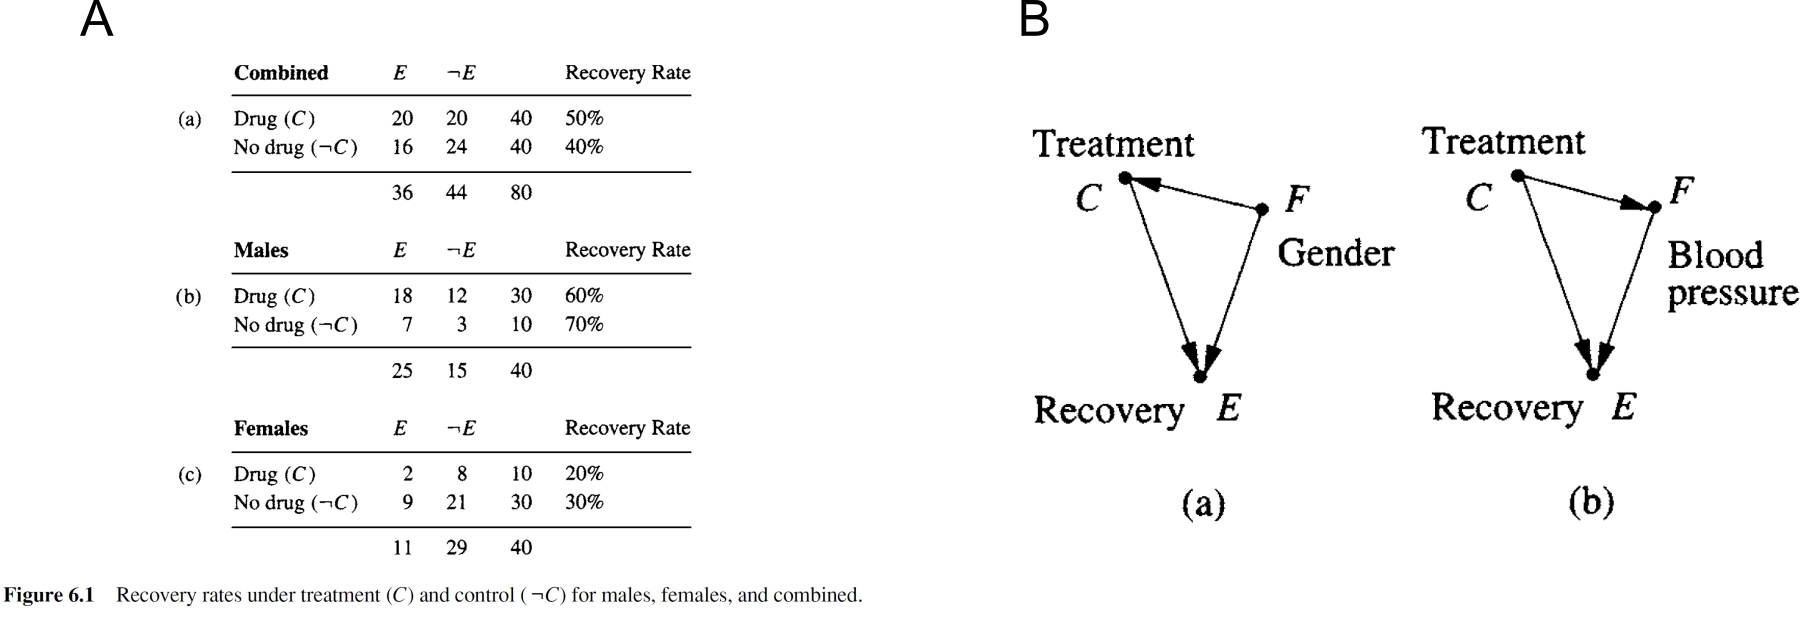
\includegraphics[width=0.8\columnwidth]{figures/simpson.png}  
\end{center}
\caption{\textbf{Example of Simpson's paradox}. A. The recovery rate in the pooled population is greater with the drug, but for both the male and female populations the recovery rate is greater without the drug. B. Two causal models which are observationally equivalent capable of generating the data in (A). In (A), $P(E|do(C)) = \sum_F P(E|C,F) P(F)$  (Theorem~\ref{thm:back-door-adjustment}) which averages over sub-populations, whereas in (B), $P(E|do(C)) = P(E|C)$ (Theorem~\ref{thm:do-calc-act-obs-ex}) which uses the pooled data.
}
\label{Fig:simpson}
\end{figure}

An example dataset displaying Simpson's paradox is in Fig.~\ref{Fig:simpson} for a drug treatment ($C$), recovery ($E$), for sub-populations of gender ($F$). The question, therefore, is: "what is the total effect of the drug on recovery?". The solution to this question depends on the causal assumptions we bring to bear on the problem: two different causal models which are capable of generating the data yield different answers for the quantity $P(E|do(C))$, one of which averages over the subpopulations, and the other using pooled data. 

\begin{thm}[Sure-thing Principle]
An action $C$ that increases the probability of an event $E$ in each sub-population $F$ must also increase the probability of $E$ in the population as a whole, provided that the action does not change the distribution of the sub-populations. In other words, for dichotomous sub-populations $F$, if  \label{thm:sure-thing}
\begin{align}
P(E|do(C), F) &< P(E|do(\neg C), F) \\
P(E|do(C), \neg F) &< P(E|do(\neg C), \neg F) \nonumber
\end{align}
then
\begin{equation}
P(E|do(C)) < P(E|do(\neg C))
\end{equation}
\end{thm}

Theorem~\ref{thm:sure-thing} follows from do-calculus, and gives the intuitive result that if the drug in Fig.~\ref{Fig:simpson}A harms both men and women then one should not administer the drug if one does not know the patient's gender, despite the fact that the observational conditional densities obey $P(E|C)>P(E|\neg C)$. The ``paradox'' in the example arises because the males, who recover (regardless of the drug) more often than the females, are also more likely than the females to use the drug.

\subsection{Confounding}

\begin{defn}[No confounding] \label{def:no-confounding}
Variables $X$ and $Y$ are not confounded in a causal model $M$ if and only if
\begin{equation}
P(y|do(x)) = P(y|x),\ \text{or}\ P(x|do(y)) = P(x|y)
\end{equation}
for all $x$ and $y$ in their respective domains. If this condition holds, we say $P(x|y)$ is unbiased. 
\end{defn}

Note that no confounding is a special case of exogeneity under a theory $T$ of the set of all models with a given DAG (see Definition~\ref{def:general-exog}). 

\begin{thm}[Common-cause principle]
Let $A_D$ be the set of assumptions embedded in an acyclic causal diagram $D$. Variables $X$ and $Y$ are stably unconfounded given $A_D$ if and only if $X$ and $Y$ have no common ancestor in $D$.
\end{thm}

The following theorem is an operational test for stable no-confounding (i.e. no confounding for every parametrization of the causal diagram):
\begin{thm}[Criterion for stable no-confounding]\label{thm:no-conf-criterion}
Let $A_Z$ denote the assumptions that (i) the data are generated by some (unspecified) acyclic model $M$ and (ii) $Z$ is a variable in $M$ that is unaffected by $X$, but does contain a directed path from $Z$ to $Y$, and so $Z$ may possibly affect $Y$. If both of the following conditions are \textbf{violated}:
\begin{enumerate}[noitemsep]
\item $P(x|z)=P(x)$ (i.e. no association between $Z$ and $X$)
\item $P(y|z,x)=P(y|x)$ (i.e. $Z$ is not associated with $Y$ conditional on $X$)
\end{enumerate}
then $(X,Y)$ are \textbf{not} stably unconfounded given $A_Z$. I.e. finding \textbf{any} variable $Z$ that satisfies $A_Z$ and violates both of the conditions above permits us to disqualify $(X,Y)$ as stably unconfounded.
\end{thm}

\subsection{Collapsibility and confounding}
\begin{defn}
Let $g[P(x,y)]$ be any functional that measures an association between $X$ and $Y$ in the joint distribution $P(x,y)$. We say that $g$ is collapsible on a variable $Z$ if 
\begin{equation}
E_z g[P(x,y|z)] = g[P(x,y)]
\end{equation}
\end{defn}

If $g$ stands for any linear functional of $P(y|x)$, such as the risk difference $P(y|x_1) - P(y|x_2)$, then collapsibility holds whenever $Z \indep X$ or $Z \indep Y| X$. Hence, any violation of collapsibility implies violation of the two statistical conditions in Theorem~\ref{thm:no-conf-criterion}. So whilst collapsibility is linked to confounding, in the absence of the assumptions $A_z$, collapsibility is neither necessary nor sufficient.

\section{Structure-based counterfactuals}
\subsection{Definitions}\label{sec:counterfactual-defs}
Let's begin by writing Eq.\eqref{eq:func-caus-mod} more formally:

\begin{defn}[Structural Causal Model] \label{defn:struct-causal-model}
A causal model is a triple
\begin{equation}
M = \langle U, V, F \rangle \nonumber
\end{equation}
where
\begin{enumerate}[noitemsep]
\item $U$ is a set of background (exogenous, or error) variables, that are determined by factors outside the model;
\item $V$ is a set $\{V_1, V_2,..., V_n \}$ of (endogenous) variables, that are determined by variables in the model -- that is, variables in $U \cup V$; and
\item $F$ is a set of functions $\{f_1, f_2,...,f_n \}$ such that each $f_i$ is a mapping from (the respective domains of) $U_i \cup PA_i$, where $U_i \subseteq U$ and $PA_i \subseteq V \setminus V_i$ and the entire set $F$ forms a mapping from $U$ to $V$. In other words, each $f_i$ in
\begin{equation}
v_i = f_i(pa_i, u_i), \ i=1,...,n \label{eq:structural-equations}
\end{equation}
assigns a value to $V_i$ that depends on (the values of) a select set of variables in $V \cup U$, and the entire set $F$ has a unique solution $V(u)$.
\end{enumerate}
\end{defn}

Uniqueness is ensured in recursive systems (acyclic, see Defn.~\ref{def:recursiveness}), but multiple solutions are allowed in non-recursive systems. Every causal model $M$ can be associated with a graph $G(M)$ called a \textbf{causal diagram} where nodes are variables and directed edges point from members of $PA_i$ and $U_i$ towards $V_i$. $G(M)$ identifies the endogenous and background variables that have direct influence on each $V_i$, but not the functional form $f_i$. The convention of confining the parent set $PA_i$ to variables in $V$ stems from the fact that the background variables are often unobservable.

\begin{defn}[Submodel]
Let $M$ be a causal model, $X$ a set of variables in $V$, and $x$ a particular realization of $X$. A submodel $M_x$ of $M$ is the causal model
\begin{equation}
M_x = \langle U, V, F_x \rangle, \nonumber
\end{equation}
where
\begin{equation}
F_x = \{f_i : V_i \notin X \} \cup \{X=x \}
\end{equation}
I.e. $F_x$ is formed by deleting from $F$ all functions $f_i$ corresponding to members of set $X$ and replacing them with the set of constant functions $X=x$.
\end{defn}

\begin{defn}[Effect of action]
Let $M$ be a causal model, $X$ a set of variables in $V$, and $x$ a particular realization of $X$. The effect of action $do(X=x)$ on $M$ is given by the submodel $M_x$.
\end{defn}

\begin{defn}[Potential response]
Let $X$ and $Y$ be two subsets in $V$. The potential response of $Y$ to action $do(X=x)$, denoted $Y_x(u)$, is the solution for $Y$ of the set of equations $F_x$. That is, $Y_x(u) = Y_{M_x}(u)$. If $Y$ is a set of variables $Y=(Y_1,Y_2,...)$ then $Y_x(u) = (Y_{1_x},Y_{2_x},...)$.
\end{defn}

\begin{defn}[Counterfactual]
Let $X$ and $Y$ be two subsets of variables in $V$. The counterfactual sentence ``$Y$ would be $y$ in situation $u$, had $X$ been x'' is interpreted as the equality $Y_x(u)=y$, with $Y_x(u)$ being the potential response of $Y$ to $X=x$.
\end{defn}

\begin{defn}[Probabilistic causal model]
A probabilistic causal model is a pair
\begin{equation}
\langle M, P(u)\rangle \nonumber
\end{equation}
where $M$ is a causal model and $P(u)$ is a probability function defined over the domain of the background variables $U$.
\end{defn}

The function $P(u)$, together with $f_i$, defines a probability distribution over endogenous variables
\begin{equation}
P(y) \defeq P(Y=y) = \sum_{\{u|Y(u)=y\}} P(u)
\end{equation}
and counterfactual probabilities are defined in a similar model through the function $Y_x(u)$ induced by submodel $M_x$:
\begin{equation}
P(Y_x=y) = P(Y=y) = \sum_{\{u|Y_x(u)=y\}} P(u).
\end{equation}
Similarly, one can define joint densities over counterfactuals and observations over (not necessarily disjoint) sets of variables
\begin{align}
P(Y_x=y, X=x') &= \sum_{\{u|Y_x(u)=y\ \&\ X(u)=x'\}} P(u) \\
P(Y_x=y, Y_{x'}=y') &= \sum_{\{u|Y_x(u)=y\ \&\ Y_{x'}(u)=y'\}} P(u)
\end{align}

We may interpret statements like ``the probability that $X=x$ was the cause of event $Y=y$'' using the counterfactual statement ``the probability that $Y$ would not be equal to $y$ had it not been for $X=x$, given that $X=x$ and $Y=y$ have in fact occurred''. We can write this counterfactual as a conditional on observations
\begin{align}
P(Y_{x'}=y'| X=x, Y=y) &= \frac{P(Y_{x'}=y', X=x, Y=y)}{P(X=x, Y=y)} \\
&= \sum_u P(Y_{x'}(u) = y')P(u|x, y).
\end{align}
In other words, we use the observations to update $P(u)$ to $P(u|x,y)$, and then use this update to compute the expectation of the equality $Y_{x'}=u$ [\textbf{TODO: Clarify after Ch~9}]. This substantiates the three-step procedure discussed in Section~/\ref{sec:counterfactuals-example}, summarized in the following theorem:
\begin{thm}[Computation of counterfactual statements] \label{thm:comp-counterfactuals}
Given model $\langle M, P(u)\rangle$, the conditional probability $P(B_A|e)$ of a counterfactual statement ``If it were $A$ then $B$'', given observational evidence $e$, can be evaluated using the following three steps:
\begin{enumerate}[noitemsep]
\item \textbf{Abduction} -- Update $P(u)$ by the evidence $e$ to obtain $P(u|e)$. (Abduction means reasoning from evidence to explanation)
\item \textbf{Action} -- Modify $M$ by the action $do(A)$, where $A$ is the antecedent of the counterfactual, to obtain submodel $M_A$.
\item \textbf{Prediction} -- Use the modified model $\langle M_A, P(u|e)\rangle$ to compute the probability of $B$, the consequence of the counterfactual.
\end{enumerate}
\end{thm}

\begin{defn}[Connection between causal effect and counterfactual]
\begin{equation}
P(Y|do(x)) \defeq P(Y_{x}=y)
\end{equation}
\end{defn}

\begin{defn}[Worlds and theories]
A causal world $w$ is a pair $\langle M,u \rangle$, where $M$ is a causal model and $u$ is a particular realization of the background variables $U=u$ (i.e.\ $P(u)=1$). A causal theory is a set of causal worlds.
\end{defn}

The crucial difference between counterfactual statements and a statement about actions, is that \textbf{in counterfactual statements, the facts (i.e. the evidence) can potentially be affected by the antecedents}. For example, in the two-man firing squad example, ``If the prisoner is dead [evidence], then the prisoner would be dead even if rifleman $A$ had not shot [antecedent]''. In this sentence, the fact that the prisoner is dead could be affected by the fact that $A$ did not shoot. This is not the case for statements about actions. For example, ``If the captain gave no signal [evidence] and rifleman $A$ decides to shoot [antecedent], then the prisoner will die and $B$ will not shoot''. Here, the evidence that the captain gives no signal is not affected by the antecedent that $A$ shoots. In natural language, counterfactual utterances tend to presume knowledge of facts that are affected by the antecedent. For example ``$O$ would be different were it not for $A$'' implies knowledge of the actual value of $O$, and that $O$ is susceptible to $A$. In general, some knowledge of the functional mechanisms of $f_i(pa_i, u_i)$ are necessary to evaluate such statements.

In a more general sense, causal effects tend to be concepts based on \textit{general} causes (e.g. ``Drinking hemlock causes death''), whereas counterfactuals tend to be concepts based on \textit{singular} causes (e.g.\ ``Socrates' drinking hemlock caused his death''). The latter (counterfactuals) tends to require access to more detailed, mechanistic, specifications and higher computational resources than the former (generic causes). Formally, the difference hinges on whether we need to condition our beliefs on the cause/effect events that actually occurred. 

\subsection{Twin network representation}
A difficulty in Theorem~\ref{thm:comp-counterfactuals} is the need to compute, store, and use the posterior distribution $P(u|e)$. This difficulty can be avoided using the twin network representation for counterfactual computation. We replicate the endogenous variables and label them distinctly, share the exogenous variables, and amputate edges of the twin network to represent the antecedent of the counterfactual. Given a counterfactual query $P(Y_x=y|z)$ for arbitrary $X$, $Y$, and $Z$, it is sufficient to compute $P(y^*|z)$ which can be performed by standard evidence propagation techniques, rather than computing the full posterior distribution $P(u|e)$ -- see Fig.~\ref{Fig:twin-network}. The twin representation is also useful for testing independencies between counterfactual quantities by testing $d$-separation (Defn.~\ref{defn:d-sep}).

\begin{figure}
\begin{center}
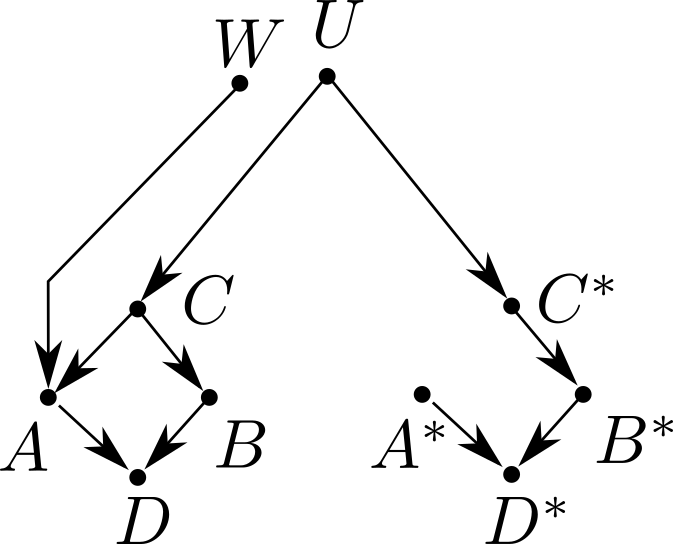
\includegraphics[width=0.4\columnwidth]{figures/twin-network.png}  
\end{center}
\caption{\textbf{Twin network representation of (semi-deterministic) firing squad problem}. A court $U$ issues an order to captain $C$ to execute a prisoner, with some probability. Upon receiving an order, the captain instructs both riflemen $A$ and $B$ to fire. Rifleman $A$ is of a nervous disposition ($W$), causing him to fire randomly (and independently of the order), with some probability. The prisoner dies if either $A$ or $B$ opens fire. Consider the counterfactual query: ``Given that the prisoner is dead, what is the probability that the prisoner would be alive if $A$ did not shoot?'', i.e. $P(\neg D_{\neg A}| D)$. This can be answered without reference to $P(u,w|D)$, only the ordinary conditional probability $P(\neg D^*|D)$, using the twin network representation. }
\label{Fig:twin-network}
\end{figure}

\subsection{Simon's causal ordering}

In general, a physical law need not be specified as a system of structural equations (Eq.\ref{eq:structural-equations}), but as a set of functional constraints
\begin{equation}
G_k(x_1,...,x_l; u_1,...,u_m) = 0
\end{equation}
without identifying a `dependent' variable (positivism: where all descriptions of Nature are defined through `functiona relations' and `interdependence' amongst variables). This seems to be at odds with the notion of causation.

\cite{Simon77} devised a procedure for deciding whether a collection of such functions $G_k$ dictates a unique way of selecting an endogenous dependent variable for each mechanism $G_k$. The procedure involves finding an order of variables $(X_1,...,X_n)$ such that we can solve for each $X_i$ without solving for any of $X_i$'s successor. If such an ordering exists, it dictates the direction of causal attribution. The ordering is unique if one can find a unique one-to-one correspondence between equations $G$ and variables $X$. If the matching is unique, then the choice of dependent variable is unique and defines a DAG \citep{Nayak94}. This means that the problem of causal induction can be reduced to the more familiar problem of scientific induction.

\subsection{Axioms of structural counterfactuals}
We present three properties of counterfactuals -- composition, effectiveness, and reversibility -- that hold in all causal models.

\begin{prop}[Composition] \label{prop:composition}
For any three sets of endogenous variables $X$, $Y$, and $W$ in a causal model, we have
\begin{equation}
W_x(u) = w \implies\ Y_{xw}(u) = Y_x(u)
\end{equation}
\end{prop}

Composition states that, if we force a variable ($W$) to a value $w$ that it would have had without our intervention, then the intervention will have no effect on other variables ($Y$) in the system. That invariance holds for all fixed conditions $do(X=x)$.

\begin{defn}[Null action]
\begin{equation}
Y_{\emptyset}(u) \defeq Y(u) \nonumber
\end{equation}
\end{defn}

\begin{cor}[Consistency]  
For any set of variables $Y$ and $X$ in a causal model,
\begin{equation}
X(u)=x \implies\ Y(u) = Y_x(u) \label{eq:consistency}
\end{equation}
\end{cor}
In other words, if we force variable $X$ to take the value it would have naturally had, then a counterfactual is equivalent to the observational value.

\begin{prop}[Effectiveness] \label{prop:effectiveness}
For all sets of variables $X$ and $W$,
\begin{equation}
X_{xw}(u) = x.
\end{equation}
\end{prop} 
Effectiveness states that if we force a variable $X$ to have the value $x$, then $X$ will indeed take on the value $x$.

\begin{prop}[Reversibility] \label{prop:reversibility}
For any two variables $Y$ and $W$, and any set of variables $X$
\begin{equation}
(Y_{xw}(u)=y)\ \&\ (W_{xy}(u)=w) \implies Y_x(u)=y
\end{equation}
\end{prop}
Reversibility precludes multiple solutions due to feedback loops. If setting $W$ to a value $w$ results in a value $y$ for $Y$, and if setting $Y$ to the value $y$ results in $W$ achieving the value $w$, then $W$ and $Y$ will naturally obtain the values $w$ and $y$, without any external setting. This holds for all fixed conditions $do(X=x)$. Reversibility, as an axiom, is only required for non-recursive systems (see Defn.~\ref{def:recursiveness} below): i.e.\ directed acyclic graphs only need composition and effectiveness to certify all truth statements.

Properties \ref{prop:composition}, \ref{prop:effectiveness}, and \ref{prop:reversibility} hold in all causal models -- they are necessary and sufficient axioms for all causal statements. In other words, if we can reduce a counterfactual quantity $Q$ into an expression that involves only ordinary probabilities using these three axioms, then $Q$ is identifiable. If $Q$ cannot be reduced in terms of ordinary probabilities using these three axioms, then $Q$ is unidentifiable. The axioms are as powerful as can be.

\begin{defn}[Recursiveness] \label{def:recursiveness}
Let $X$ and $Y$ be singleton variables in a model, and let $X \rightarrow Y$ stand for the inequality $Y_{xw}(u) \neq Y_w(u)$ for some values of $x$, $w$, and $u$. A model $M$ is recursive if, for any sequence $X_1, X_2, ..., X_k$, we have
\begin{equation}
X_1 \rightarrow X_2,\ X_2 \rightarrow X_3,\ ...,\ X_{k-1} \rightarrow X_k \implies X_k \nrightarrow X_1
\end{equation}
\end{defn}

Properties \ref{prop:composition}, \ref{prop:effectiveness}, and Defn.~\ref{def:recursiveness} are complete: i.e. in a recursive system, only composition and effectiveness are needed to derive all causal statements. Property~\ref{prop:reversibility} is only required in non-recursive systems.


\subsubsection{Rules of inference with counterfactuals (potential outcomes framework)}

The following two rules can be used to embody recursiveness
\begin{rle}[Exclusion restrictions] \label{rle:exclusion-restriction}
For every variable $Y$ having parents $PA_Y$ and for every set of variables $Z \subset V$ disjoint of $PA_Y$, we have
\begin{equation}
Y_{pa_Y}(u) = Y_{pa_Y, z}(u)
\end{equation}
\end{rle} 
Rule~\ref{rle:exclusion-restriction} reflects the insensitivity of $Y$ to any manipulation in $V$, once its direct causes $PA_Y$ are held constant.

\begin{rle}[Independence restrictions]\label{rle:independence-restriction}
If $Z_1, ..., Z_k$ is any set of nodes in $V$ not connected to $Y$ via paths containing only $U$ variables, we have
\begin{equation}
Y_{pa_Y} \indep \{Z_{1_{pa_{Z_1}}}, ..., Z_{k_{pa_{Z_k}}}\} \label{eq:independence-restriction}
\end{equation}
where $Z_{i_{pa_{Z_i}}}$ is the potential response of the variable $Z_i$ to setting the parents of $Z_i$ to the value $pa_{Z_i}$. Equivalently, Eq.~\ref{eq:independence-restriction} holds if the corresponding $U$ terms $(U_{Z_1}, ..., U_{Z_k})$ are jointly independent of $U_Y$.
\end{rle}
Rule~\ref{rle:independence-restriction} interprets independencies among $U$ variables as independencies between the counterfactuals of the corresponding $V$ variables. This is because, since $Y=f_y(pa_Y, u_Y)$, holding $PA_Y$ fixed means that the residual variations of $Y$ are entirely governed by variations in $U_Y$.

Using Rules~\ref{rle:exclusion-restriction}, \ref{rle:independence-restriction}, and Properties~\ref{prop:composition} and \ref{prop:effectiveness}, can be used to compute any causal query in a DAG.

\subsubsection{Causal relevance}
Causal relevance is concerned with questions of the form: ``Given that $Z$ is fixed, wold changing $X$ alter $Y$?''. Causal relevance can be useful when exact causal models do not exist, but constraints about the lack of influence of certain variables on others are known.

\begin{defn}[Causal irrelevance]
A variable $X$ is causally irrelevant to $Y$, given $Z$ (written $X \nrightarrow Y|Z$) if, for every set $W$ disjoint of $X \cup Y \cup Z$, we have
\begin{equation}
\forall (u, z, x, x', w), \quad Y_{xzw}(u) = Y_{x'zw}(u)
\end{equation}
where $x$ and $x'$ are two distinct values of $X$.
\end{defn}

\begin{thm}
For any causal model, the following sentences must hold.

Weak Right Decomposition:
\begin{equation}
(X \nrightarrow YW|Z)\ \&\ (X \nrightarrow Y| ZW) \implies (X \nrightarrow Y|Z)
\end{equation}

Left Decomposition:
\begin{equation}
(XW \nrightarrow Y| Z) \implies (X \nrightarrow Y | Z)\ \&\ (W \nrightarrow Y | Z)
\end{equation}

Strong Union:
\begin{equation}
(X \nrightarrow Y | Z) \implies (X \nrightarrow Y|ZW)\ \forall W
\end{equation} 

Right Intersection:
\begin{equation}
(X \nrightarrow Y|ZW)\ \&\ (X \nrightarrow W| ZY) \implies (X \nrightarrow YW|Z)
\end{equation}

Left Intersection:
\begin{equation}
(X \nrightarrow Y| ZW)\ \&\ (W \nrightarrow Y | ZX) \implies (XW \nrightarrow Y| Z)
\end{equation}
where $(X \nrightarrow Y| Z)_G$ has the interpretation that every directed path from $X$ to $Y$ in a directed graph $G$ contains at least on node in $Z$.
\end{thm}

\section{Imperfect experiments: bounding causal effects and counterfactuals}
It is not always possible to conduct perfect randomized clinical trials, for e.g. ethical or pragmatic reasons. Sometimes, we must admit a latent common cause ($U$) of the treatment a patient actually receives ($X$) and the outcome for that patient ($Y$). We have seen above that, in such a graph $X \leftarrow U \rightarrow Y$, $P(y|do(x))$ is unidentifiable. However, we may consider an instrumental variable $Z \rightarrow X$, which may count as e.g. a physician's encouragement to participate in a particular way in the study, see Fig.~\ref{Fig:partial-compliance-instrument}A. If $Z$ is assigned randomly, then we will be able to form bounds (as opposed to precise point-estimates) on $P(y|do(x))$.


\begin{figure}
\begin{center}
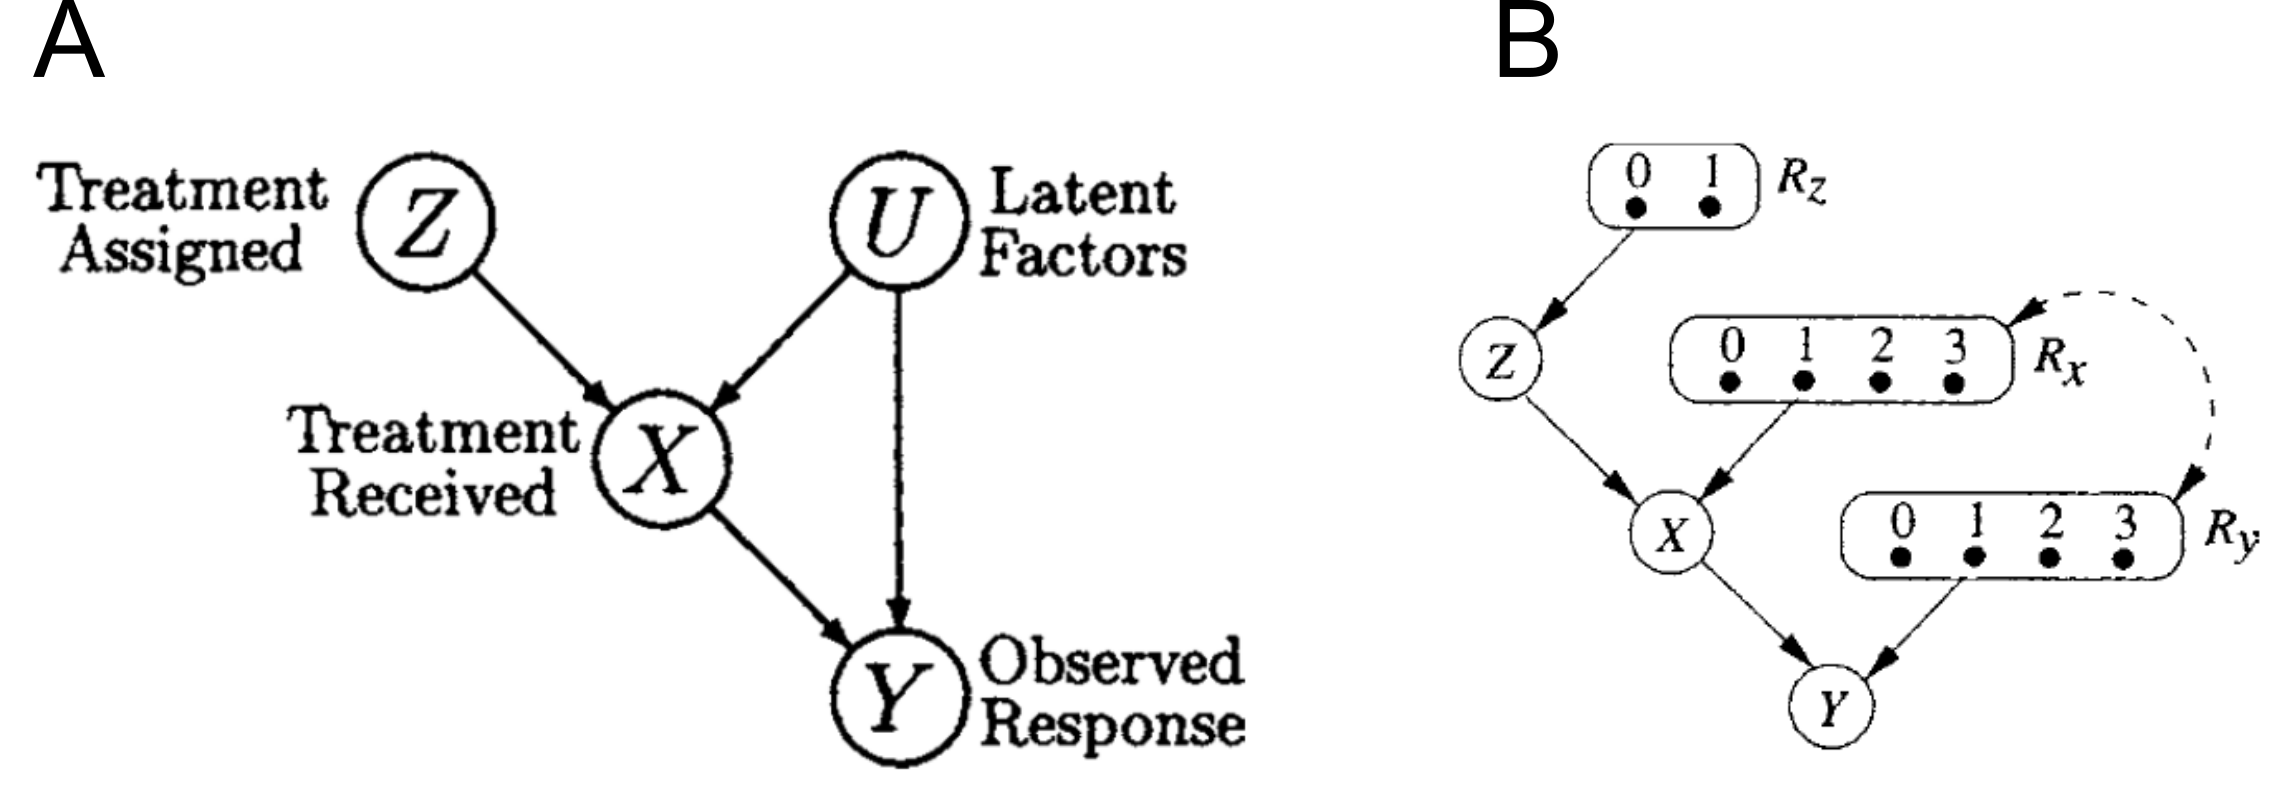
\includegraphics[width=0.8\columnwidth]{figures/partial-compliance-instrument.png}  
\end{center}
\caption{\textbf{A randomized clinical trial with partial compliance and an instrumental variable}. A. We cannot always conduct perfectly randomized clinical trials. We may bound causal effects by using an instrumental variable, such as treatment assigned. B. For binary $X$, $Y$, and $Z$, (B) is equivalent to (A), which uses finite-state response variables $R_x$, $R_y$, and $R_z$. $R_x$ and $R_y$ substitute $U$ and may, in general, be dependent.}
\label{Fig:partial-compliance-instrument}
\end{figure}

\subsection{Average causal effect}

Let $X$, $Y$, and $Z$ be binary random variables and the subscript $i$ denote an outcome for the corresponding variable, where $i \in \{0,1\}$.
\begin{defn}[Average causal effect]
The average causal effect $\text{ACE}(X\rightarrow Y)$ is defined as
\begin{equation}
\text{ACE}(X\rightarrow Y) = P(y_1|do(x_1)) - P(y_1|do(x_0))
\end{equation}
\end{defn}

Using Rule~\ref{rle:do-calc-act-obs-ex} of do-calculus,
\begin{equation}
\text{ACE}(X\rightarrow Y) = \sum_u [P(y_1|x_1, u) - P(y_1|x_0,u)]P(u). \label{eq:ace-instrument}
\end{equation}
We seek to perform a constrained optimization of finding the highest and lowest values of Eq.~\eqref{eq:ace-instrument}, in terms of the observed probabilities $P(y,x|z_0)$ and $P(y,x|z_1)$. 

\subsection{Canonical partitions}
No matter the form of $y=f(x,u)$, since $Y$ and $X$ are binary, we can always partition the domain of $U$ into four equivalence classes
\begin{align}
f_0: y=0,\quad f_1: y=x \\
f_1: y = \neg x, \quad f_2: y=1. \nonumber
\end{align}
Therefore for any $P(u)$ there exists a $P(r),\ r=0, 1, 2, 3$ which is given by the total weight assigned to the equivalence class corresponding to $f_r$. Since $X$, $Y$ and $Z$ are all binary variables, the state space of $U$ divides into $4\times 2 + 4\times 2 = 16$ equivalence classes, since $U$ affects both $X$ and $Y$. For convenience, we can split the state space into two four-valued variables $R_x$ and $R_y$. We can then write, e.g.
\begin{equation}
x=f_X(z,r_x)=\begin{cases}
x_0& \text{if}\ r_x=0;\\
x_0& \text{if}\ r_x=1\ \text{and}\ z=z_0;\\
x_1& \text{if}\ r_x=1\ \text{and}\ z=z_1;\\
x_1& \text{if}\ r_x=2\ \text{and}\ z=z_0;\\
x_0& \text{if}\ r_x=2\ \text{and}\ z=z_1;\\
x_1& \text{if}\ r_x=3.
\end{cases}
\end{equation}
We can call subjects with compliance behaviour $r_x=0, 1, 2, 3$ as \textit{never-taker}, \textit{complier}, \textit{defier}, and \textit{always-taker}. We can define a similar mapping for $y=f_Y(x,r_y)$ with $r_y=0, 1, 2, 3$ corresponding to \textit{never-recover}, \textit{helped}, \textit{hurt}, and \textit{always-recover} (see Fig.~\ref{Fig:partial-compliance-instrument}B). The counterfactual $Y_{x_0}$ may be written as
\begin{equation}
Y_{x_0} = \begin{cases}
y_1& \text{if}\ r_y=2\ \text{or}\ r_y=3, \\
y_0& \text{otherwise}
\end{cases}
\end{equation}
and similar for $Y_{x_1}$. Hence,
\begin{equation}
P(y_1|do(x_0))=P(r_y=2) + P(r_3=3).
\end{equation}
Given the definition of ACE in Eq.\eqref{eq:ace-instrument}, the conditional distribution $P(y,x|z)$, and the probabilistic constraints that $\sum_{x,y}P(x,y|z_0)=\sum_{x,y}P(x,y|z_1)=1$, one may write down $ACE(X\rightarrow Y)$ as a linear programming problem, where we seek to minimize/maximize $ACE$ given the constraints (for details see Section 8.2.3 of \cite{pearl09}). The \textbf{natural bound} yields a less tight bound, which is simpler in its form (see Section 8.2.4 of \cite{pearl09}). The width of the natural bounds is given by the rate of noncompliance: $P(x_1|z_0) + P(x_0|z_1)$. Natural bounds are optimal when no patient is a contrarian. Note that if the variables are continuous, then dichotomized variables can be defined.

Gibbs sampling can be used to infer the distribution of the average causal effect in this system by representing the joint distribution of $(r_x, r_y)$ with a vector of length 16 denoting the probability of occupying each of the 16 possible subpopulations \citep{Chickering97}.

\subsection{Effect of treatment on the treated}
ETT is useful when we want to know the impact of the treatment \textit{on the treated}, for e.g. deciding whether to maintain/terminate a program. It is defined as 
\begin{equation}
ETT(X \rightarrow Y) \defeq P(Y_{x_1}=y_1|x_1) - P(Y_{x_0}=y_1|x_1).
\end{equation}

For the same DAG as Fig.~\ref{Fig:partial-compliance-instrument}, bounds may be derived through a similar means as the above (see \citep{pearl09}). Under conditions of \textit{no intrusion} (i.e.\ $P(x_1|z_0)=0$), $ETT(X \rightarrow Y)$ can be identified precisely, and is
\begin{equation}
ETT(X\rightarrow Y) = \frac{P(y_1|z_1) - P(y_1|z_0)}{P(x_1|z_1)}.
\end{equation}

\subsection{Test for instruments}
Casting the estimation of $ACE(X\rightarrow Y)$ as a linear programming problem can allow us to derive tests for whether a variable $Z$ is a plausible instrumental variable: i.e. a variable which is exogenous relative to $P(y|do(x))$. The following inequalities follow, by asserting that the upper bound of $ACE$ is greater than the lower bound
\begin{align}
P(y_0, x_0|z_0) + P(y_1, x_0| z_1) &\leq 1, \nonumber \\
P(y_0, x_1|z_0) + P(y_1, x_1| z_1) &\leq 1, \nonumber \\
P(y_1, x_0|z_0) + P(y_0, x_0| z_1) &\leq 1, \nonumber \\
P(y_1, x_1|z_0) + P(y_0, x_1| z_1) &\leq 1.
\end{align}
Violation of any of these inequalities implies that $Z$ cannot be an instrumental variable. This is not guaranteed to screen out all violations of exogeneity, but may still be useful. Generalizations for multivalued, and continuous $Z$ or $Y$ are
\begin{align}
\max_x \sum_y [\max_z P(y, x|z)] \leq 1 \\
\int_y \max_z[f(y|x,z)P(x|z)] dy \leq 1\ \forall x
\end{align}
respectively. These are called the \textbf{instrumental inequality}. Interestingly, for continuous $X$, Fig.~\ref{Fig:partial-compliance-instrument} places no constraint on the observed density whatsoever.

\section{Probability of causation: Interpretation and Identification}

\subsection{Definitions}

\begin{defn}[Probability of Necessity, PN]
Let $X$ and $Y$ be two binary variables in a causal model $M$. Let $x$ and $y$ stand (respectively) for the propositions $X=$ true and $Y=$ true, and $x'$ and $y'$ denote their complements. The probability of necessity is defined as the expression
\begin{equation}
\text{PN} \defeq P(Y_{x'}=\text{false}\ | X=\text{true}, Y=\text{true}) \defeq P(y'_{x'}|x,y).
\end{equation}
\end{defn}
\noindent i.e.\ PN stands for the probability that $y$ would not have occurred if $x$ had not occurred, given that $x$ and $y$ did in fact occur. Note the slight change of notation where $y_x \iff Y_x=\text{true}$.

\begin{defn}[Probability of Sufficiency, PS]
\begin{equation}
\text{PS} \defeq P(y_x|y',x')
\end{equation}
\end{defn}
\noindent i.e.\ PS stands for the probability that $y$ would have happened if $x$ had occurred, given that neither $x$ nor $y$ did in fact occur. PS measures the capacity of $x$ to \textit{produce} $y$, and since ``production'' implies a transition from the absence to the presence of $x$ and $y$, we condition on $x'$ and $y'$. In other words, it is the probability of $x$ causing $y$ in worlds where all other causes of $y$ are suppressed, or a ``causal power'' of $x$ over $y$.

\begin{defn}[Probability of Necessity and Sufficiency, PNS]
\begin{equation}
\text{PNS} \defeq P(y_x, y'_{x'})
\end{equation}
\end{defn}
\noindent i.e.\ PNS stands for the probability that $y$ would respond to $x$ in both ways, and therefore measures both necessity and sufficiency of $x$ to produce $y$.

\begin{defn}[Probability of Disablement, PD]
\begin{equation}
\text{PD} \defeq P(y'_{x'}|y)
\end{equation}
\end{defn}
\noindent i.e.\ PD measures the probability that $y$ would have been prevented if it were not for $x$.

\begin{defn}[Probability of Enablement, PE]
\begin{equation}
\text{PE} \defeq P(y_x|y')
\end{equation}
\end{defn}
\noindent i.e.\ PE measures the probability that $y$ would have happened if $x$ were the case.

None of these quantities are sufficient for deriving the others, but they are not entirely independent.

\begin{lma}
\begin{equation}
\text{PNS} = P(x,y)\text{PN} + P(x',y')\text{PS}
\end{equation}
\end{lma}

Since $y$ is assumed to be affected by $x$, and since all of the above quantities involve conditionalization on $y$, none of these quantities is identifiable from knowledge of the causal diagram and the data alone, even under conditions of no-confounding. However, given the assumption of no confounding (\textit{exogeneity}), useful bounds and relationships can be derived.

\subsection{Bounds and relationships under exogeneity}

\begin{defn}[Strong exogeneity]
A variable $X$ is exogenous (in a strong sense) relative to $Y$ in model $M$ if and only if
\begin{equation}
\{Y_x, Y_{x'}\} \indep X
\end{equation}
where $\{Y_x, Y_{x'}\}$ is a joint variable. In other words, the way $Y$ would potentially respond to conditions $x$ or $x'$ is independent of the actual value of $X$.
\end{defn}

Translating the consistency property Eq.\eqref{eq:consistency} into $x \implies (y_x=y)$, then strong exogeneity allows us to write
\begin{equation}
P(y_x) = P(y_x|x) = P(y|x) \label{eq:strong-identifiability}
\end{equation}
where the first step requires strong exogeneity, and the second uses Eq.\eqref{eq:consistency}. This is also called ``strong identifiability''.

\begin{thm}[Bound for PNS]
Under strong exogeneity, PNS is bounded as 
\begin{equation}
\max[0, P(y|x) - P(y|x')] \leq \text{PNS} \leq min[P(y|x), P(y'|x')]
\end{equation}
\end{thm}

Using Eq.~\eqref{eq:strong-identifiability} with the above bound gives bounds on PN and PS through the relations
\begin{align}
\text{PN}&=\frac{\text{PNS}}{P(y|x)} \label{eq:pn-exog}\\
\text{PS}&=\frac{\text{PNS}}{P(y'|x')} \label{eq:ps-exog}
\end{align}

\subsection{Identifiability under monotonicity and exogeneity}
The special condition of monotonicity expresses the assumption that a change from $X=$ false to $X=$ true cannot, under any circumstances, make $Y$ change from true to false. In epidemiology, this is often expressed as ``no prevention'', that is, no individual in the population can be helped by exposure to the risk factor.
\begin{defn}[Monotonicity]
A variable $Y$ is monotonic relative to variable $X$ in a causal model $M$ if and only if 
\begin{equation}
y_x' \wedge y_{x'}=\ \text{false}
\end{equation}
\end{defn}

\begin{thm}[Identifiability under exogeneity and monotonicity]
If $X$ is exogenous and $Y$ is monotonic relative to $X$ then the probabilities PN, PS, and PNS are all identifiable and are given by Eq.\eqref{eq:pn-exog} and Eq.\eqref{eq:ps-exog}, along with
\begin{equation}
\text{PNS}=P(y|x) - P(y|x') \label{eq:pns-exog-mono}
\end{equation}
\end{thm}
\noindent The RHS of Eq.\eqref{eq:pns-exog-mono} is called ``\textbf{risk difference}''. 

Given the assumptions of monotonicity and exogeneity, PN given by
\begin{equation}
\text{PN}=\frac{P(y|x)-P(y|x')}{P(y|x)}
\end{equation}
and is called the ``\textbf{excess risk ratio}'', and measures the fraction of exposed cases that are attributable to the exposure. Likewise, PS is given by
\begin{equation}
\text{PS}=\frac{P(y|x)-P(y|x')}{1-P(y|x')}
\end{equation}
and is called by epidemiologists the ``\textbf{susceptibility}'' of a population to an exposure $x$. It measures the proportion of individuals who possess ``an underlying factor sufficient to make a person contract a disease following exposure''.

\subsection{Identifiability under monotonicity and non-exogeneity}
Now consider when the effect of $X$ on $Y$ is confounded, i.e. $P(y_x)\neq P(y|x)$. 
\begin{thm}
If $Y$ is monotonic relative to $X$, then PNS, PN, and PS are identifiable whenever the causal effects $P(y_x)$ and $P(y_{x'})$ are identifiable
\begin{align}
\text{PNS} &= P(y_x)-P(y_{x'}) \\
\text{PN} &= \frac{P(y)-P(y_{x'})}{P(x,y)} \\
\text{PS} &= \frac{P(y_x)-P(y)}{P(x',y')} \\
\end{align}
\end{thm}
If we can e.g. perform an experiment to identify $P(y_x)$ and $P(y_{x'})$, then we can access PNS/PN/PS.

\begin{thm}[Test for monotonicity]
Since PN and PS are non-negative, the assumption of monotonicity implies
\begin{equation}
P(y_x) \geq P(y) \geq P(y_{x'})
\end{equation}
\end{thm}

\subsection{Example: Betting against a fair coin}
Consider a fair coin where $u$ denotes an outcome of heads, $x$ is betting on heads, and $y$ is winning the bet. Then
\begin{equation}
y=(x \wedge u) \vee (x' \wedge u').
\end{equation}
Plugging into our definitions of PN, PS, and PNS, we arrive at PN$=1$, PS$=1$, and PNS$=1/2$. In other words, betting heads has a 50\% chance of being a necessary and sufficient cause of winning; once we win we can be 100\% sure that our bet was necessary for our win, and once we lose we are 100\% sure that betting heads would have produced a win. Such counterfactuals cannot be recovered from merely $P(X,Y)$ because the probabilities
\begin{equation}
P(y|x) = P(y|x') = P(y_x) = P(y_{x'}) = P(y) = 1/2
\end{equation}
would also be recovered from a random payoff policy where $y$ is functionally independent of $x$ -- say by a bookie who makes a random payout regardless of our bet. The three probabilities of causation cannot be inferred from observational data alone, nor even controlled experiment. Knowledge of the functional relationship must be used these counterfactuals. Note that whether the coin is tossed before or after the bet is placed has no bearing on the probabilities of causation, in contrast to some other theories of causation.

\section{Software}

\subsection{Tetrad}
\begin{itemize}[noitemsep]
\item Allows you to build causal graphs, a variety of parametric models (Bayesian causal graphs, SEMs,...), instantiate them with particular parametrizations
\item Allows you to do model search, given data. Can be combined to create a ground truth, simulate, then do inference, all inside the same environment
\item Implemented as a Java GUI
\item Available for download \href{https://www.ccd.pitt.edu/tools/}{here} 
\item Manual here \href{http://cmu-phil.github.io/tetrad/manual/}{here}
\end{itemize}

\subsection{\texttt{causaleffect}} \label{sec:soft-causaleffect}
\begin{itemize}[noitemsep]
\item Build causal graphs, and perform do-calculus to identify causal effects in terms of observational densities \cite{tikka17}, see Fig.~\ref{Fig:graph_cond_ci}
\item Implemented in an \texttt{R} package, \texttt{causaleffect}
\item Jupyter Notebook example \href{https://github.com/jaryaman/ML_demos/blob/master/Notebooks/do-calculus.ipynb}{here}
\item Does not return a causal effect in its simplest form
\end{itemize}

\section*{Acknowledgements}
Thanks to Aidan Marshall for many useful conversations on the topic of causal inference. 

\newpage
\bibliography{causality.bib} 

\end{document}